% Chương 2
\chapter[\MakeUppercase{Phân tích và thiết kế hệ thống}]{Phân tích và thiết kế hệ thống}
\label{ch:chuong2}

% TODO: chỉ có khung mục. Chương này mô tả thiết kế theo kiến trúc microservice bám sát hiện trạng code (gồm 6 service: gateway, identity, consultation, clinical, knowledge, ai).
% Nội dung bản cũ lưu ở chuong2/luu_tru/chuong2_noi_dung_cu.tex (không được nạp vào main.tex).

\section{Phân tích yêu cầu}

\subsection{Tác nhân và yêu cầu của hệ thống}

Trong hệ thống hỗ trợ tiền chẩn đoán và tư vấn bệnh da liễu, các tác nhân (actors) tham gia tương tác trực tiếp hoặc gián tiếp với hệ thống được xác định bao gồm: Người dùng, Bệnh nhân, Bác sĩ và Quản trị viên. Thông tin và vai trò của từng tác nhân được mô tả chi tiết trong Bảng~\ref{tab:tac-nhan}.

\begin{longtable}{|>{\raggedright\arraybackslash}p{0.08\dimexpr\linewidth-6\tabcolsep\relax}|>{\raggedright\arraybackslash}p{0.18\dimexpr\linewidth-6\tabcolsep\relax}|>{\raggedright\arraybackslash}p{0.74\dimexpr\linewidth-6\tabcolsep\relax}|}
\caption{Các tác nhân của hệ thống}\label{tab:tac-nhan}\\
\hline
\textbf{STT} & \textbf{Tên tác nhân} & \textbf{Mô tả vai trò và yêu cầu tương tác} \\ \hline
\endfirsthead
\hline
\textbf{STT} & \textbf{Tên tác nhân} & \textbf{Mô tả vai trò và yêu cầu tương tác} \\ \hline
\endhead
1 & Người dùng & Là người dùng hệ thống đã được đăng ký tài khoản và đăng nhập vào ứng dụng, có quyền quản lý tài khoản của mình và thực hiện đăng xuất. \\ \hline
2 & Bệnh nhân & Là người sử dụng hệ thống để nhận hỗ trợ tiền chẩn đoán và trao đổi thông tin về bệnh da liễu:
\begin{itemize}[leftmargin=*,nosep]
  \item Hỏi đáp với chatbot, gửi hình ảnh tổn thương da và mô tả triệu chứng để nhận dự đoán và khuyến nghị sơ bộ.
  \item Tra cứu thông tin bệnh lý, các ca bệnh tương tự từ Knowledge Base và đặt lịch khám với bác sĩ chuyên khoa.
  \item Xem và quản lý hồ sơ bệnh án, lịch sử khám và các hình ảnh bệnh đã lưu trữ của bản thân hoặc người thân.
  \item Trao đổi trực tiếp với bác sĩ thông qua kênh chat hoặc cuộc gọi video (video call). Trong trường hợp bác sĩ chưa tiếp nhận ngay, bệnh nhân tiếp tục trao đổi với chatbot.
  \item Thông tin từ cuộc trò chuyện với chatbot được hệ thống tự động tổng hợp thành dữ kiện lâm sàng (\textit{clinical facts}) và báo cáo hỗ trợ bác sĩ trước khi tư vấn.
\end{itemize} \\ \hline
3 & Bác sĩ & Là người sử dụng hệ thống để tiếp nhận, thăm khám, tư vấn và quản lý thông tin bệnh nhân:
\begin{itemize}[leftmargin=*,nosep]
  \item Xem báo cáo tổng hợp tự động trước khi thực hiện thăm khám lâm sàng.
  \item Xem các dữ kiện lâm sàng (\textit{clinical facts}), nguồn lập luận trích xuất từ Knowledge Base, lịch sử bệnh án và hồ sơ bệnh nhân.
  \item Chỉnh sửa, cập nhật hồ sơ sau mỗi lượt khám; lưu trữ ca bệnh và hình ảnh đã được xác nhận để làm dữ liệu tham khảo và phục vụ phát triển mô hình CNN.
  \item Trao đổi trực tiếp với bệnh nhân qua chat hoặc video call; truy xuất tin nhắn nguồn làm bằng chứng cho từng kết luận.
  \item Trực quan hóa Đồ thị tri thức bệnh nhân (\textit{Patient Journey Knowledge Graph - PJKG}) liên quan.
  \item Tải lên giáo trình, guideline và tài liệu y khoa để bổ sung vào Knowledge Base; phối hợp với trợ lý AI để tra cứu và làm giàu cơ sở tri thức.
\end{itemize} \\ \hline
4 & Quản trị viên & Quản lý người dùng, kiểm duyệt danh sách và thông tin bác sĩ, theo dõi và vận hành các pipeline dữ liệu của hệ thống. \\ \hline
\end{longtable}

\subsection{Biểu đồ use case tổng quan}

Dựa trên các tác nhân và yêu cầu nghiệp vụ đã xác định, biểu đồ use case tổng quan của hệ thống được thể hiện trong Hình~\ref{fig:usecase_tong_quan}.

\begin{figure}[H]
  \centering
  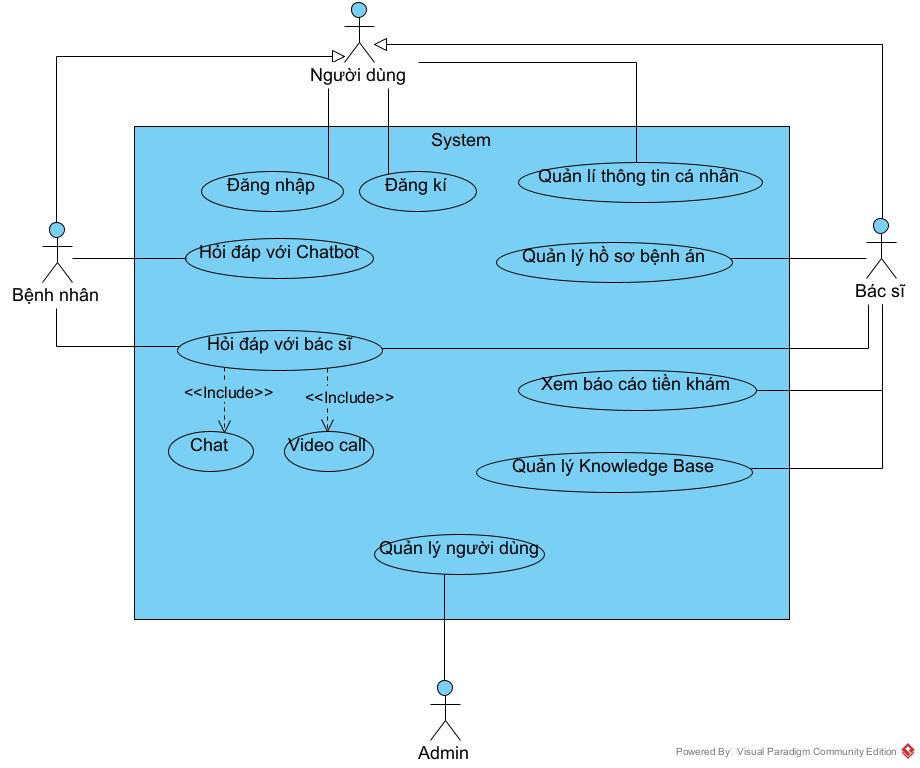
\includegraphics[width=0.95\linewidth,height=0.7\textheight,keepaspectratio]{chuong2/hinh/usecase_tong_quan.jpg}
  \caption{Sơ đồ use case tổng quan của hệ thống}
  \label{fig:usecase_tong_quan}
\end{figure}

Hệ thống được chia thành các nhóm chức năng chính bao gồm:
\begin{itemize}
  \item \textbf{Usecase Đăng ký (Sign Up):} Cho phép người dùng mới tạo tài khoản trên hệ thống với vai trò tương ứng (bệnh nhân hoặc bác sĩ).
  \item \textbf{Usecase Đăng nhập (Sign In):} Xác thực danh tính người dùng (sử dụng JWT token) để truy cập vào các chức năng tương ứng với quyền hạn của mình.
  \item \textbf{Usecase Quản lý thông tin cá nhân (Profile Management):} Cho phép xem, cập nhật và chỉnh sửa thông tin cá nhân, liên hệ, chuyên môn (đối với bác sĩ) hoặc quản lý nhiều hồ sơ y tế thành viên trong gia đình (đối với bệnh nhân).
  \item \textbf{Usecase Quản lý người dùng (User Administration):} Dành cho quản trị viên nhằm kiểm tra, phê duyệt hồ sơ bác sĩ và kiểm soát trạng thái hoạt động của các tài khoản.
\end{itemize}

\subsection{Use case chi tiết}

Phần này trình bày kịch bản chuẩn và các ngoại lệ cho từng use case chính của hệ thống theo mẫu use case chi tiết (use case, tác nhân, tiền/hậu điều kiện, kịch bản chính và ngoại lệ). Biểu đồ use case chi tiết cho từng use case được bổ sung riêng. Trong các kịch bản, hệ thống được gọi chung là ``hệ thống''; các giá trị cụ thể (tên đăng nhập, mật khẩu, dữ liệu mẫu) lấy từ tài khoản demo.

\subsubsection{UC1: Đăng ký và đăng nhập}

\begin{figure}[H]
  \centering
  
\includegraphics[width=0.4\linewidth,keepaspectratio]{chuong2/hinh/dang_nhap.jpg}
  \caption{Sơ đồ use case chi tiết -- UC1: Đăng ký và đăng nhập}
  \label{fig:uc1}
\end{figure}

Chức năng đăng nhập/đăng ký có các giao diện tương tác với người dùng:

\begin{itemize}[nosep,leftmargin=*]
  \item Đăng nhập/đăng ký -> Đề xuất UC đăng nhập/đăng ký
\end{itemize}

Như vậy, biểu đồ UC chi tiết cho modul đăng nhập/đăng ký được trình bày trong Hình trên. Các UC được mô tả như sau:

\begin{itemize}[nosep,leftmargin=*]
  \item \textbf{Đăng nhập/đăng ký}: UC này cho phép người dùng thực hiện đăng nhập hoặc đăng ký tài khoản để truy cập vào hệ thống.
\end{itemize}

% bảng use case giãn dòng như văn bản: tắt giãn dòng đơn mặc định của longtable
\renewcommand{\tablespacing}{}
\begin{spacing}{1.5}
\renewcommand{\arraystretch}{1.15}
\begin{longtable}{|>{\raggedright\arraybackslash}p{0.18\textwidth}|>{\raggedright\arraybackslash}p{0.77\textwidth}|}
\hline
\textbf{Use case} & Đăng ký / Đăng nhập \\ \hline
\textbf{Tác nhân} & Người dùng (Bệnh nhân, Bác sĩ, Quản trị viên) \\ \hline
\textbf{Tiền điều kiện} & Chưa đăng nhập vào hệ thống. \\ \hline
\textbf{Hậu điều kiện} & Người dùng được xác thực, nhận cặp token (Access Token, Refresh Token) và chuyển vào giao diện tương ứng với vai trò. \\ \hline
\textbf{Kịch bản chính} &
\begin{enumerate}[nosep,leftmargin=*]
  \item Người dùng mở ứng dụng, giao diện đăng nhập hiện lên với hai ô ``Tên đăng nhập'' và ``Mật khẩu'' cùng nút ``Đăng nhập''.
  \item Nhập tên đăng nhập = \texttt{user-1}, mật khẩu = \texttt{123456}, nhấn ``Đăng nhập''; hệ thống kiểm tra tên đăng nhập tồn tại và so khớp mật khẩu (bcrypt).
  \item Hệ thống phát hành Access Token (JWT, 30 phút) và Refresh Token (30 ngày), lưu Refresh Token trên Redis.
  \item Client lưu token và chuyển vào giao diện theo vai trò.
\end{enumerate} \\ \hline
\textbf{Ngoại lệ} &
\begin{itemize}[nosep,leftmargin=2.6em,labelwidth=2em,labelsep=0.5em,align=left]
  \item[2.] Hệ thống báo đăng nhập không thành công (sai mật khẩu hoặc tài khoản không tồn tại).
  \begin{itemize}[nosep,leftmargin=3em,labelwidth=2.4em,labelsep=0.4em,align=left]
    \item[2.1] Người dùng click ``OK'' của thông báo.
    \item[2.2] Hệ thống hiện giao diện đăng nhập: username = \texttt{user-1}, password = (trống).
    \item[2.3] Người dùng sửa lại mật khẩu thành \texttt{123456}, click ``Đăng nhập''.
    \item[2.4] Giao diện chính của bệnh nhân hiện lên.
  \end{itemize}
  \item[4.] Token hết hạn.
  \begin{itemize}[nosep,leftmargin=3em,labelwidth=2.4em,labelsep=0.4em,align=left]
    \item[4.1] Client dùng Refresh Token để lấy Access Token mới.
    \item[4.2] Nếu Refresh Token hết hạn, hệ thống bắt buộc đăng nhập lại (về bước 1).
  \end{itemize}
\end{itemize} \\ \hline
\end{longtable}
\end{spacing}

\subsubsection{UC2: Hỏi đáp với chatbot tiền chẩn đoán}

\begin{figure}[H]
  \centering
  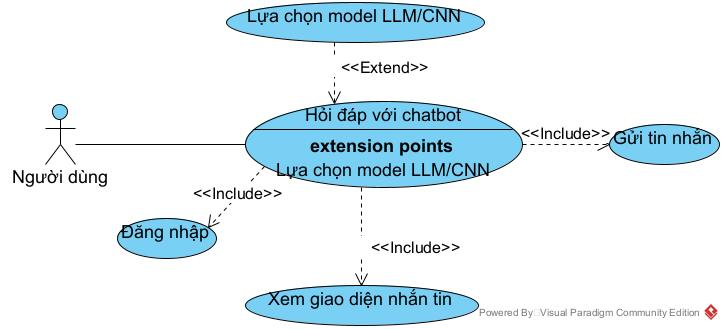
\includegraphics[width=0.95\linewidth,height=0.7\textheight,keepaspectratio]{chuong2/hinh/hoi_dap_chatbot.jpg}
  \caption{Sơ đồ use case chi tiết -- UC2: Hỏi đáp với chatbot tiền chẩn đoán}
  \label{fig:uc2}
\end{figure}

Chức năng hỏi đáp với chatbot tiền chẩn đoán có các giao diện tương tác với người dùng:

\begin{itemize}[nosep,leftmargin=*]
  \item Đăng nhập -> Đề xuất UC đăng nhập
\end{itemize}

\begin{itemize}[nosep,leftmargin=*]
  \item Xem giao diện nhắn tin -> Đề xuất UC xem giao diện nhắn tin
\end{itemize}

\begin{itemize}[nosep,leftmargin=*]
  \item Lựa chọn model LLM/CNN -> Đề xuất UC lựa chọn model LLM/CNN
\end{itemize}

\begin{itemize}[nosep,leftmargin=*]
  \item Gửi tin nhắn -> Đề xuất UC gửi tin nhắn
\end{itemize}

Như vậy, biểu đồ UC chi tiết cho modul hỏi đáp với chatbot tiền chẩn đoán được trình bày trong Hình trên. Các UC được mô tả như sau:

\begin{itemize}[nosep,leftmargin=*]
  \item \textbf{Xem giao diện nhắn tin}: UC này cho phép người dùng xem giao diện trò chuyện chính với chatbot.
\end{itemize}

\begin{itemize}[nosep,leftmargin=*]
  \item \textbf{Lựa chọn model LLM/CNN}: UC này cho phép người dùng tùy chọn mô hình trí tuệ nhân tạo (LLM hoặc CNN) phù hợp để phục vụ cho quá trình hỏi đáp.
\end{itemize}

\begin{itemize}[nosep,leftmargin=*]
  \item \textbf{Gửi tin nhắn}: UC này cho phép người dùng nhập nội dung câu hỏi và gửi đi để nhận phản hồi từ chatbot.
\end{itemize}

\begin{spacing}{1.5}
\renewcommand{\arraystretch}{1.15}
\begin{longtable}{|>{\raggedright\arraybackslash}p{0.18\textwidth}|>{\raggedright\arraybackslash}p{0.77\textwidth}|}
\hline
\textbf{Use case} & Hỏi đáp với chatbot tiền chẩn đoán \\ \hline
\textbf{Tác nhân} & Bệnh nhân, Hệ thống AI \\ \hline
\textbf{Tiền điều kiện} & Bệnh nhân đã đăng nhập và có hồ sơ bệnh nhân. \\ \hline
\textbf{Hậu điều kiện} & Tin nhắn và kết quả tiền chẩn đoán được lưu; các dữ kiện lâm sàng (\textit{clinical facts}) được trích xuất sang hệ thống lâm sàng. \\ \hline
\textbf{Kịch bản chính} &
\begin{enumerate}[nosep,leftmargin=*]
  \item Bệnh nhân mở giao diện chat, chọn model LLM (mặc định Gemma 4 26B) và model CNN (mặc định EfficientNet-B0).
  \item Bệnh nhân nhập mô tả: ``Da mặt nổi nhiều mụn đỏ, ngứa 3 ngày nay'' và đính kèm 1 ảnh tổn thương.
  \item Hệ thống lưu tin nhắn người dùng (kèm \texttt{attached\_files}), tạo tin nhắn assistant (\texttt{status = queued}).
  \item Hệ thống gửi yêu cầu lượt chạy sang tác nhân AI.
  \item Tác nhân AI gọi mô hình CNN để phân loại ảnh, trả về top-5 nhãn kèm \% tin cậy (ví dụ: Acne 82\%, Rosacea 9\%).
  \item Tác nhân AI gọi công cụ tìm kiếm ngữ nghĩa và tra cứu đồ thị tri thức để đối chiếu guideline y khoa.
  \item Tác nhân AI tự động bóc tách các dữ kiện lâm sàng (vị trí: mặt; thời gian: 3 ngày; triệu chứng: ngứa; mức độ: đỏ).
  \item Tác nhân AI stream câu trả lời về giao diện theo thời gian thực (SSE): giải thích tham khảo, khuyến cáo mức độ cấp bách, hướng xử trí.
  \item Kết thúc lượt, hệ thống ghi nhận dữ kiện lâm sàng vào hồ sơ bệnh nhân.
  \item Bệnh nhân xem kết quả tiền chẩn đoán mang tính tham khảo cùng khuyến cáo mức độ cấp bách.
\end{enumerate} \\ \hline
\textbf{Ngoại lệ} &
\begin{itemize}[nosep,leftmargin=2.6em,labelwidth=2em,labelsep=0.5em,align=left]
  \item[5.] Ảnh không tải được từ kho lưu trữ.
  \begin{itemize}[nosep,leftmargin=3em,labelwidth=2.4em,labelsep=0.4em,align=left]
    \item[5.1] Agent báo ``Không tìm thấy ảnh'', tiếp tục xử lý phần văn bản.
    \item[5.2] Hệ thống vẫn stream câu trả lời dựa trên mô tả văn bản.
  \end{itemize}
  \item[8.] LLM hoặc dịch vụ tri thức lỗi.
  \begin{itemize}[nosep,leftmargin=3em,labelwidth=2.4em,labelsep=0.4em,align=left]
    \item[8.1] Agent trả thông báo lỗi, tin nhắn assistant chuyển trạng thái \texttt{done} với nội dung lỗi.
    \item[8.2] Bệnh nhân có thể gửi lại tin nhắn.
  \end{itemize}
\end{itemize} \\ \hline
\end{longtable}
\end{spacing}

\subsubsection{UC3: Đặt lịch hẹn và tiếp nhận lần khám}

\begin{figure}[H]
  \centering
  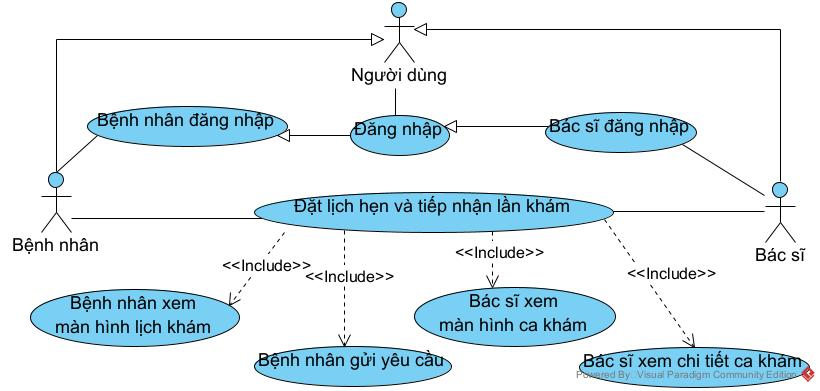
\includegraphics[width=0.95\linewidth,height=0.7\textheight,keepaspectratio]{chuong2/hinh/dat_lich_hen.jpg}
  \caption{Sơ đồ use case chi tiết -- UC3: Đặt lịch hẹn và tiếp nhận lần khám}
  \label{fig:uc3}
\end{figure}

Chức năng đặt lịch hẹn và tiếp nhận lần khám có các giao diện tương tác với bệnh nhân và bác sĩ:

\begin{itemize}[nosep,leftmargin=*]
  \item Đăng nhập (Bệnh nhân đăng nhập, Bác sĩ đăng nhập) -> Đề xuất UC đăng nhập (UC bệnh nhân đăng nhập, UC bác sĩ đăng nhập)
\end{itemize}

\begin{itemize}[nosep,leftmargin=*]
  \item Bệnh nhân xem màn hình lịch khám -> Đề xuất UC bệnh nhân xem màn hình lịch khám
\end{itemize}

\begin{itemize}[nosep,leftmargin=*]
  \item Bệnh nhân gửi yêu cầu -> Đề xuất UC bệnh nhân gửi yêu cầu
\end{itemize}

\begin{itemize}[nosep,leftmargin=*]
  \item Bác sĩ xem màn hình ca khám -> Đề xuất UC bác sĩ xem màn hình ca khám
\end{itemize}

\begin{itemize}[nosep,leftmargin=*]
  \item Bác sĩ xem chi tiết ca khám -> Đề xuất UC bác sĩ xem chi tiết ca khám
\end{itemize}

Như vậy, biểu đồ UC chi tiết cho modul đặt lịch hẹn và tiếp nhận lần khám được trình bày trong Hình trên. Các UC được mô tả như sau:

\begin{itemize}[nosep,leftmargin=*]
  \item \textbf{Bệnh nhân xem màn hình lịch khám}: UC này cho phép bệnh nhân xem thông tin về các lịch khám hiện có trên hệ thống.
\end{itemize}

\begin{itemize}[nosep,leftmargin=*]
  \item \textbf{Bệnh nhân gửi yêu cầu}: UC này cho phép bệnh nhân điền thông tin và gửi yêu cầu đặt lịch hẹn khám bệnh.
\end{itemize}

\begin{itemize}[nosep,leftmargin=*]
  \item \textbf{Bác sĩ xem màn hình ca khám}: UC này cho phép bác sĩ theo dõi danh sách các ca khám được đăng ký.
\end{itemize}

\begin{itemize}[nosep,leftmargin=*]
  \item \textbf{Bác sĩ xem chi tiết ca khám}: UC này cho phép bác sĩ xem thông tin chi tiết của một ca khám cụ thể để thực hiện tiếp nhận lần khám.
\end{itemize}

\begin{spacing}{1.5}
\renewcommand{\arraystretch}{1.15}
\begin{longtable}{|>{\raggedright\arraybackslash}p{0.18\textwidth}|>{\raggedright\arraybackslash}p{0.77\textwidth}|}
\hline
\textbf{Use case} & Đặt lịch hẹn và tiếp nhận lần khám \\ \hline
\textbf{Tác nhân} & Bệnh nhân, Bác sĩ \\ \hline
\textbf{Tiền điều kiện} & Bệnh nhân đã đăng nhập; đợt bệnh của hồ sơ đang mở, chưa quá hạn, đã có giả thuyết của AI và chưa có lịch hẹn còn hiệu lực; bác sĩ đã đăng nhập. \\ \hline
\textbf{Hậu điều kiện} & Lịch hẹn (\texttt{Appointment}) được tạo và được bác sĩ xác nhận; lần khám (\texttt{Encounter}, trạng thái \texttt{open}) được tạo, đợt bệnh chuyển \texttt{in\_exam}, kênh trao đổi bác sĩ -- bệnh nhân được mở. \\ \hline
\textbf{Kịch bản chính} &
\begin{enumerate}[nosep,leftmargin=*]
  \item Bệnh nhân Nguyễn Văn An bấm mục ``Lịch khám'' ở sidebar của giao diện.
  \item Hệ thống hiện màn hình ``Lịch khám'' với 2 tab ``Đang theo dõi'' và ``Lịch hẹn''.
  \item Tab ``Đang theo dõi'' hiện danh sách các vấn đề bệnh nhân đang gặp. Mỗi dòng hiện tên vùng da, thời gian cập nhật, tóm tắt dữ kiện và nút ``Đặt lịch''.
  \item Bệnh nhân bấm ``Đặt lịch'' ở dòng vùng chân (ngứa rát kèm vài mảng đỏ ở cẳng chân).
  \item Hệ thống hiện hộp thoại ``Đặt lịch · Chân'' gồm ô chọn thời gian, ô lý do (không bắt buộc) và nút ``Gửi yêu cầu''.
  \item Bệnh nhân chọn thời gian 08:00 ngày 26/11/2026, nhập lý do rồi bấm ``Gửi yêu cầu''.
\end{enumerate} \\ \cline{2-2}
\textbf{Kịch bản chính (tiếp)} &
\begin{enumerate}[nosep,leftmargin=*,start=7]
  \item Hệ thống kiểm tra điều kiện đặt lịch, tạo lịch hẹn ở trạng thái ``Chờ'', hiện thông báo ``Đã gửi yêu cầu đặt lịch''; dòng vùng chân đổi nút ``Đặt lịch'' thành trạng thái ``Chờ'', tab ``Lịch hẹn'' thêm dòng ``Chân · 26/11/2026 08:00'' kèm dòng phụ ``Chờ bác sĩ nhận'', trạng thái ``Chờ'' và nút ``Huỷ''.
  \item Bác sĩ bấm mục ``Ca khám'' ở sidebar của giao diện.
  \item Hệ thống hiện giao diện ``Ca khám'' gồm bộ lọc trạng thái, ô ``Tìm bệnh nhân'' và bảng các ca khám.
  \item Bác sĩ xem danh sách ca khám, bấm nút ``Xác nhận lịch'' (dấu $\checkmark$) ở dòng của bệnh nhân Nguyễn Văn An.
  \item Hệ thống đổi trạng thái ca khám thành ``Đã hẹn'' và gán bác sĩ cho lịch; phía bệnh nhân, dòng lịch hiện ``BS. Trần Thị Bình'' thay cho ``Chờ bác sĩ nhận''.
  \item Bác sĩ bấm nút ``Bắt đầu khám'' (dấu $\blacktriangleright$): hệ thống đổi trạng thái thành ``Đang khám'' và mở kênh trao đổi bác sĩ -- bệnh nhân.
  \item Hệ thống mở trang ``Chi tiết ca khám'' kèm bản tổng hợp tiền khám: dữ kiện lâm sàng, giả thuyết AI và bằng chứng trích từ chat, ảnh tổn thương kèm dự đoán CNN, lịch sử khám.
  \item Bác sĩ trao đổi thêm với bệnh nhân ở khung ``Trao đổi với bệnh nhân'' và chuẩn bị buổi khám.
\end{enumerate} \\ \hline
\textbf{Ngoại lệ} &
\begin{itemize}[nosep,leftmargin=2.6em,labelwidth=2em,labelsep=0.5em,align=left]
  \item[7.] Không tạo được lịch hẹn: đợt bệnh đã có lịch hẹn còn hiệu lực, chưa đủ thông tin (chưa có giả thuyết AI), đợt bệnh đã quá hạn hoặc thời gian hẹn không ở tương lai.
  \begin{itemize}[nosep,leftmargin=3em,labelwidth=2.4em,labelsep=0.4em,align=left]
    \item[7.1] Hệ thống báo lỗi tương ứng, không tạo lịch hẹn.
    \item[7.2] Bệnh nhân huỷ lịch hẹn cũ (nhập lý do) hoặc quay lại chat mô tả thêm triệu chứng rồi đặt lại với thời gian khác.
  \end{itemize}
  \item[10.] Lịch đã được bác sĩ khác xác nhận trước đó.
  \begin{itemize}[nosep,leftmargin=3em,labelwidth=2.4em,labelsep=0.4em,align=left]
    \item[10.1] Hệ thống báo ``Chỉ xác nhận được lịch hẹn đang chờ.'', lịch đã biến khỏi bộ lọc ``Chờ xác nhận''.
    \item[10.2] Bác sĩ tải lại danh sách ca khám (chỉ bác sĩ đã nhận mới thấy lịch này).
  \end{itemize}
  \item[12.] Không bắt đầu khám được vì đợt bệnh không còn mở.
  \begin{itemize}[nosep,leftmargin=3em,labelwidth=2.4em,labelsep=0.4em,align=left]
    \item[12.1] Hệ thống báo ``Đợt bệnh không còn mở, hãy đổi sang đợt khác hoặc huỷ lịch.''
    \item[12.2] Bác sĩ đổi lịch sang đợt khác của cùng hồ sơ (khối ``Bệnh nhân có vấn đề ở vùng khác\ldots'') hoặc huỷ lịch kèm lý do; nếu bệnh nhân không đến thì đánh dấu ``Bệnh nhân không đến''.
  \end{itemize}
\end{itemize} \\ \hline
\end{longtable}
\end{spacing}

\subsubsection{UC4: Tư vấn trực tiếp và gọi video với bác sĩ}

\begin{figure}[H]
  \centering
  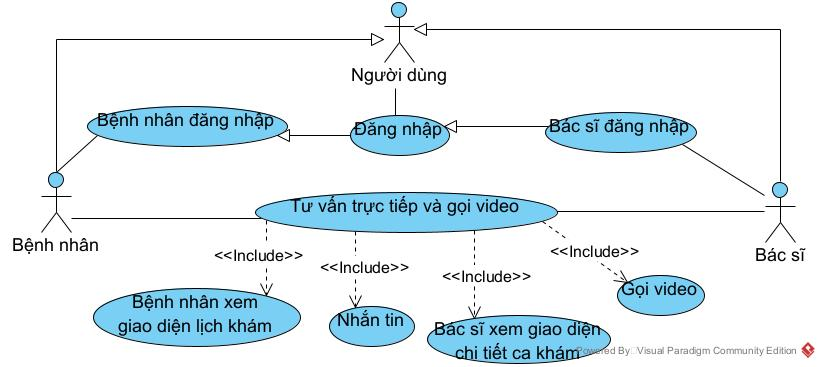
\includegraphics[width=0.95\linewidth,height=0.7\textheight,keepaspectratio]{chuong2/hinh/tu_van_truc_tiep.jpg}
  \caption{Sơ đồ use case chi tiết -- UC4: Tư vấn trực tiếp và gọi video với bác sĩ}
  \label{fig:uc4}
\end{figure}

Chức năng tư vấn trực tiếp và gọi video có các giao diện tương tác với bệnh nhân và bác sĩ:

\begin{itemize}[nosep,leftmargin=*]
  \item Đăng nhập (Bệnh nhân đăng nhập, Bác sĩ đăng nhập) -> Đề xuất UC đăng nhập (UC bệnh nhân đăng nhập, UC bác sĩ đăng nhập)
\end{itemize}

\begin{itemize}[nosep,leftmargin=*]
  \item Bệnh nhân xem giao diện lịch khám -> Đề xuất UC bệnh nhân xem giao diện lịch khám
\end{itemize}

\begin{itemize}[nosep,leftmargin=*]
  \item Bác sĩ xem giao diện chi tiết ca khám -> Đề xuất UC bác sĩ xem giao diện chi tiết ca khám
\end{itemize}

\begin{itemize}[nosep,leftmargin=*]
  \item Nhắn tin -> Đề xuất UC nhắn tin
\end{itemize}

\begin{itemize}[nosep,leftmargin=*]
  \item Gọi video -> Đề xuất UC gọi video
\end{itemize}

Như vậy, biểu đồ UC chi tiết cho modul tư vấn trực tiếp và gọi video được trình bày trong Hình trên. Các UC được mô tả như sau:

\begin{itemize}[nosep,leftmargin=*]
  \item \textbf{Bệnh nhân xem giao diện lịch khám}: UC này cho phép bệnh nhân xem giao diện thông tin lịch khám của mình.
\end{itemize}

\begin{itemize}[nosep,leftmargin=*]
  \item \textbf{Bác sĩ xem giao diện chi tiết ca khám}: UC này cho phép bác sĩ xem giao diện thông tin chi tiết của ca khám cần tư vấn.
\end{itemize}

\begin{itemize}[nosep,leftmargin=*]
  \item \textbf{Nhắn tin}: UC này cho phép bệnh nhân và bác sĩ trao đổi thông tin qua tin nhắn văn bản trực tiếp.
\end{itemize}

\begin{itemize}[nosep,leftmargin=*]
  \item \textbf{Gọi video}: UC này cho phép bệnh nhân và bác sĩ thực hiện cuộc gọi video trực tuyến để phục vụ quá trình thăm khám và tư vấn.
\end{itemize}

\begin{spacing}{1.5}
\renewcommand{\arraystretch}{1.15}
\begin{longtable}{|>{\raggedright\arraybackslash}p{0.18\textwidth}|>{\raggedright\arraybackslash}p{0.77\textwidth}|}
\hline
\textbf{Use case} & Tư vấn trực tiếp và gọi video với bác sĩ \\ \hline
\textbf{Tác nhân} & Bệnh nhân, Bác sĩ \\ \hline
\textbf{Tiền điều kiện} & Đã có cuộc hội thoại hoặc lần khám (\texttt{Encounter}) đang mở. \\ \hline
\textbf{Hậu điều kiện} & Tin nhắn và cuộc gọi video được lưu; bác sĩ quan sát tổn thương trực tiếp. \\ \hline
\textbf{Kịch bản chính} &
\begin{enumerate}[nosep,leftmargin=*]
  \item Bác sĩ và bệnh nhân trao đổi qua kênh chat: bác sĩ gửi ``Bạn có thể gửi ảnh vùng da tổn thương hiện tại không?''.
  \item Bệnh nhân gửi thêm 1 hình ảnh tổn thương qua chat.
  \item Bác sĩ khởi tạo cuộc gọi video (WebRTC); hệ thống tạo \texttt{VideoCall} (trạng thái \texttt{pending}).
  \item Bệnh nhân chấp nhận cuộc gọi; trạng thái chuyển \texttt{ongoing}, bắt đầu ghi nhận thời điểm.
  \item Hai bên trao đổi video thời gian thực: bác sĩ quan sát trực tiếp tổn thương, yêu cầu bệnh nhân xoay camera.
  \item Kết thúc cuộc gọi, trạng thái \texttt{ended}, ghi nhận thời điểm bắt đầu/kết thúc.
\end{enumerate} \\ \hline
\textbf{Ngoại lệ} &
\begin{itemize}[nosep,leftmargin=2.6em,labelwidth=2em,labelsep=0.5em,align=left]
  \item[3.] Kết nối video thất bại (mạng/firewall).
  \begin{itemize}[nosep,leftmargin=3em,labelwidth=2.4em,labelsep=0.4em,align=left]
    \item[3.1] Hệ thống báo lỗi, hai bên tiếp tục trao đổi qua tin nhắn.
    \item[3.2] Bác sĩ có thể thử gọi lại.
  \end{itemize}
  \item[5.] Mất kết nối giữa chừng.
  \begin{itemize}[nosep,leftmargin=3em,labelwidth=2.4em,labelsep=0.4em,align=left]
    \item[5.1] Trạng thái cuộc gọi chuyển \texttt{ended}.
    \item[5.2] Hai bên có thể gọi lại.
  \end{itemize}
\end{itemize} \\ \hline
\end{longtable}
\end{spacing}

\subsubsection{UC5: Chốt báo cáo kết luận và nạp ca bệnh}

\begin{figure}[H]
  \centering
  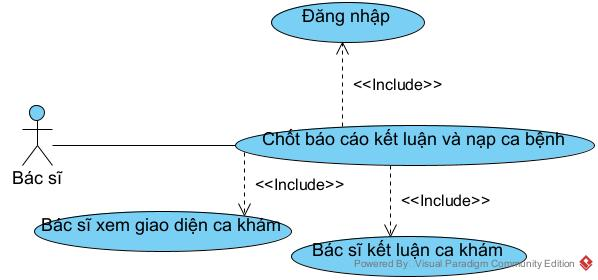
\includegraphics[width=0.95\linewidth,height=0.7\textheight,keepaspectratio]{chuong2/hinh/nap_ca_benh.jpg}
  \caption{Sơ đồ use case chi tiết -- UC5: Chốt báo cáo kết luận và nạp ca bệnh}
  \label{fig:uc5}
\end{figure}

Chức năng chốt báo cáo kết luận và nạp ca bệnh có các giao diện tương tác với bác sĩ:

\begin{itemize}[nosep,leftmargin=*]
  \item Đăng nhập -> Đề xuất UC đăng nhập
\end{itemize}

\begin{itemize}[nosep,leftmargin=*]
  \item Bác sĩ xem giao diện ca khám -> Đề xuất UC bác sĩ xem giao diện ca khám
\end{itemize}

\begin{itemize}[nosep,leftmargin=*]
  \item Bác sĩ kết luận ca khám -> Đề xuất UC bác sĩ kết luận ca khám
\end{itemize}

Như vậy, biểu đồ UC chi tiết cho modul chốt báo cáo kết luận và nạp ca bệnh được trình bày trong Hình trên. Các UC được mô tả như sau:

\begin{itemize}[nosep,leftmargin=*]
  \item \textbf{Bác sĩ xem giao diện ca khám}: UC này cho phép bác sĩ theo dõi và xem thông tin giao diện của các ca khám cần xử lý.
\end{itemize}

\begin{itemize}[nosep,leftmargin=*]
  \item \textbf{Bác sĩ kết luận ca khám}: UC này cho phép bác sĩ nhập thông tin chẩn đoán, chốt báo cáo kết luận cho ca khám và nạp dữ liệu ca bệnh vào hệ thống.
\end{itemize}

\begin{spacing}{1.5}
\renewcommand{\arraystretch}{1.15}
\begin{longtable}{|>{\raggedright\arraybackslash}p{0.18\textwidth}|>{\raggedright\arraybackslash}p{0.77\textwidth}|}
\hline
\textbf{Use case} & Chốt báo cáo kết luận và nạp ca bệnh \\ \hline
\textbf{Tác nhân} & Bác sĩ \\ \hline
\textbf{Tiền điều kiện} & Bác sĩ đã thăm khám (\texttt{Encounter} đang mở). \\ \hline
\textbf{Hậu điều kiện} & Báo cáo kết luận (\texttt{FinalizeReport}) được lưu; ca bệnh được nạp vào Knowledge Base (nếu được chọn làm ca tham khảo). \\ \hline
\textbf{Kịch bản chính} &
\begin{enumerate}[nosep,leftmargin=*]
  \item Bác sĩ nhập nhận định: ``Viêm da cơ địa (Eczema) mức độ trung bình'', hướng điều trị, ghi chú.
  \item Bác sĩ xác nhận các dữ kiện lâm sàng AI đề xuất (ngứa, đỏ, khô da) và điều chỉnh nếu cần.
  \item Hệ thống trích xuất thêm dữ kiện mới từ mô tả bác sĩ.
  \item Hệ thống lưu snapshot báo cáo kết luận (hồ sơ bệnh nhân, mức khẩn cấp, dữ kiện kèm nguồn trích dẫn).
  \item Hệ thống mở kênh theo dõi sau khám (\texttt{doctor\_followup}) với thời hạn 30 ngày.
  \item Bác sĩ đánh dấu ca bệnh tham khảo; hệ thống nạp ca bệnh vào Knowledge Base.
  \item \texttt{Encounter} chuyển trạng thái \texttt{closed}.
\end{enumerate} \\ \hline
\textbf{Ngoại lệ} &
\begin{itemize}[nosep,leftmargin=2.6em,labelwidth=2em,labelsep=0.5em,align=left]
  \item[3.] AI không trích xuất được dữ kiện.
  \begin{itemize}[nosep,leftmargin=3em,labelwidth=2.4em,labelsep=0.4em,align=left]
    \item[3.1] Bác sĩ vẫn chốt báo cáo với dữ kiện đã có.
    \item[3.2] Hệ thống lưu báo cáo bình thường.
  \end{itemize}
  \item[4.] Thiếu chẩn đoán khi đã có \texttt{Encounter}.
  \begin{itemize}[nosep,leftmargin=3em,labelwidth=2.4em,labelsep=0.4em,align=left]
    \item[4.1] Hệ thống báo lỗi.
    \item[4.2] Bác sĩ bổ sung chẩn đoán, hệ thống lưu báo cáo.
  \end{itemize}
\end{itemize} \\ \hline
\end{longtable}
\end{spacing}

\subsubsection{UC6: Số hóa giáo trình vào Knowledge Base}

\begin{figure}[H]
  \centering
  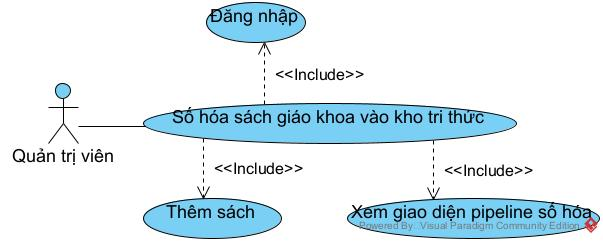
\includegraphics[width=0.95\linewidth,height=0.7\textheight,keepaspectratio]{chuong2/hinh/nap_kb.jpg}
  \caption{Sơ đồ use case chi tiết -- UC6: Số hóa giáo trình vào Knowledge Base}
  \label{fig:uc6}
\end{figure}

Chức năng số hóa sách giáo khoa vào kho tri thức có các giao diện tương tác với quản trị viên:

\begin{itemize}[nosep,leftmargin=*]
  \item Đăng nhập -> Đề xuất UC đăng nhập
\end{itemize}

\begin{itemize}[nosep,leftmargin=*]
  \item Thêm sách -> Đề xuất UC thêm sách
\end{itemize}

\begin{itemize}[nosep,leftmargin=*]
  \item Xem giao diện pipeline số hóa -> Đề xuất UC xem giao diện pipeline số hóa
\end{itemize}

Như vậy, biểu đồ UC chi tiết cho modul số hóa sách giáo khoa vào kho tri thức được trình bày trong Hình trên. Các UC được mô tả như sau:

\begin{itemize}[nosep,leftmargin=*]
  \item \textbf{Thêm sách}: UC này cho phép quản trị viên tải lên và thêm các tài liệu sách giáo khoa mới vào hệ thống để tiến hành xử lý.
\end{itemize}

\begin{itemize}[nosep,leftmargin=*]
  \item \textbf{Xem giao diện pipeline số hóa}: UC này cho phép quản trị viên theo dõi tiến trình và giao diện luồng xử lý số hóa dữ liệu sách giáo khoa vào kho tri thức.
\end{itemize}

\begin{spacing}{1.5}
\renewcommand{\arraystretch}{1.15}
\begin{longtable}{|>{\raggedright\arraybackslash}p{0.18\textwidth}|>{\raggedright\arraybackslash}p{0.77\textwidth}|}
\hline
\textbf{Use case} & Số hóa giáo trình vào Knowledge Base \\ \hline
\textbf{Tác nhân} & Quản trị viên, Knowledge Worker \\ \hline
\textbf{Tiền điều kiện} & Quản trị viên đã đăng nhập; có file PDF giáo trình. \\ \hline
\textbf{Hậu điều kiện} & Tài liệu được trích xuất, phân đoạn và nạp vector vào Qdrant; có thể truy xuất qua RAG. \\ \hline
\textbf{Kịch bản chính} &
\begin{enumerate}[nosep,leftmargin=*]
  \item Quản trị viên tải lên file PDF giáo trình da liễu (ví dụ ``Habif Clinical Dermatology.pdf'', 45 MB).
  \item Hệ thống kiểm tra file PDF hợp lệ (bắt đầu bằng \texttt{\%PDF}, kích thước $\le$ 500 MB), tạo bản ghi \texttt{Document} và 4 bước (\texttt{ingest}, \texttt{toc}, \texttt{chunks}, \texttt{index}) ở trạng thái \texttt{not\_started}.
  \item Knowledge Worker thực thi bước \textit{ingest}: trích xuất văn bản từng trang, lưu \texttt{pages.jsonl} vào MinIO.
  \item Người duyệt xem kết quả, nhấn \texttt{approve}; bước chuyển \texttt{approved}.
  \item Knowledge Worker thực thi bước \textit{toc}: AI nhận diện cấu trúc mục lục, trả về cây mục; người duyệt chỉnh sửa (\textit{override}) nếu cần, rồi \texttt{approve}.
  \item Knowledge Worker thực thi bước \textit{chunks}: phân đoạn văn bản theo mục lục, lưu \texttt{chunks.jsonl}.
  \item Knowledge Worker thực thi bước \textit{index}: sinh vector nhúng (OpenRouter) và nạp vào Qdrant.
  \item Tài liệu sẵn sàng phục vụ truy xuất ngữ nghĩa cho tác nhân AI.
\end{enumerate} \\ \hline
\textbf{Ngoại lệ} &
\begin{itemize}[nosep,leftmargin=2.6em,labelwidth=2em,labelsep=0.5em,align=left]
  \item[2.] File không phải PDF hoặc vượt 500 MB.
  \begin{itemize}[nosep,leftmargin=3em,labelwidth=2.4em,labelsep=0.4em,align=left]
    \item[2.1] Hệ thống từ chối upload, báo lỗi.
    \item[2.2] Người dùng chọn file khác và tải lại.
  \end{itemize}
  \item[3.] Một bước thất bại.
  \begin{itemize}[nosep,leftmargin=3em,labelwidth=2.4em,labelsep=0.4em,align=left]
    \item[3.1] Trạng thái \texttt{failed}, thông báo lỗi hiển thị nguyên văn.
    \item[3.2] Người duyệt sửa tham số và chạy lại.
  \end{itemize}
\end{itemize} \\ \hline
\end{longtable}
\end{spacing}
\renewcommand{\tablespacing}{\singlespacing}
\section{Thiết kế thực thể}

\subsection{Các lớp thực thể liên quan}

Để hiện thực hóa các yêu cầu nghiệp vụ của hệ thống, sơ đồ lớp tổng thể được thiết kế nhằm mô hình hóa đầy đủ các đối tượng thực thể và mối liên kết giữa chúng. Sơ đồ lớp tổng quan của hệ thống được biểu diễn trong Hình~\ref{fig:so_do_lop}.

\begin{sidewaysfigure}[p]
  \centering
  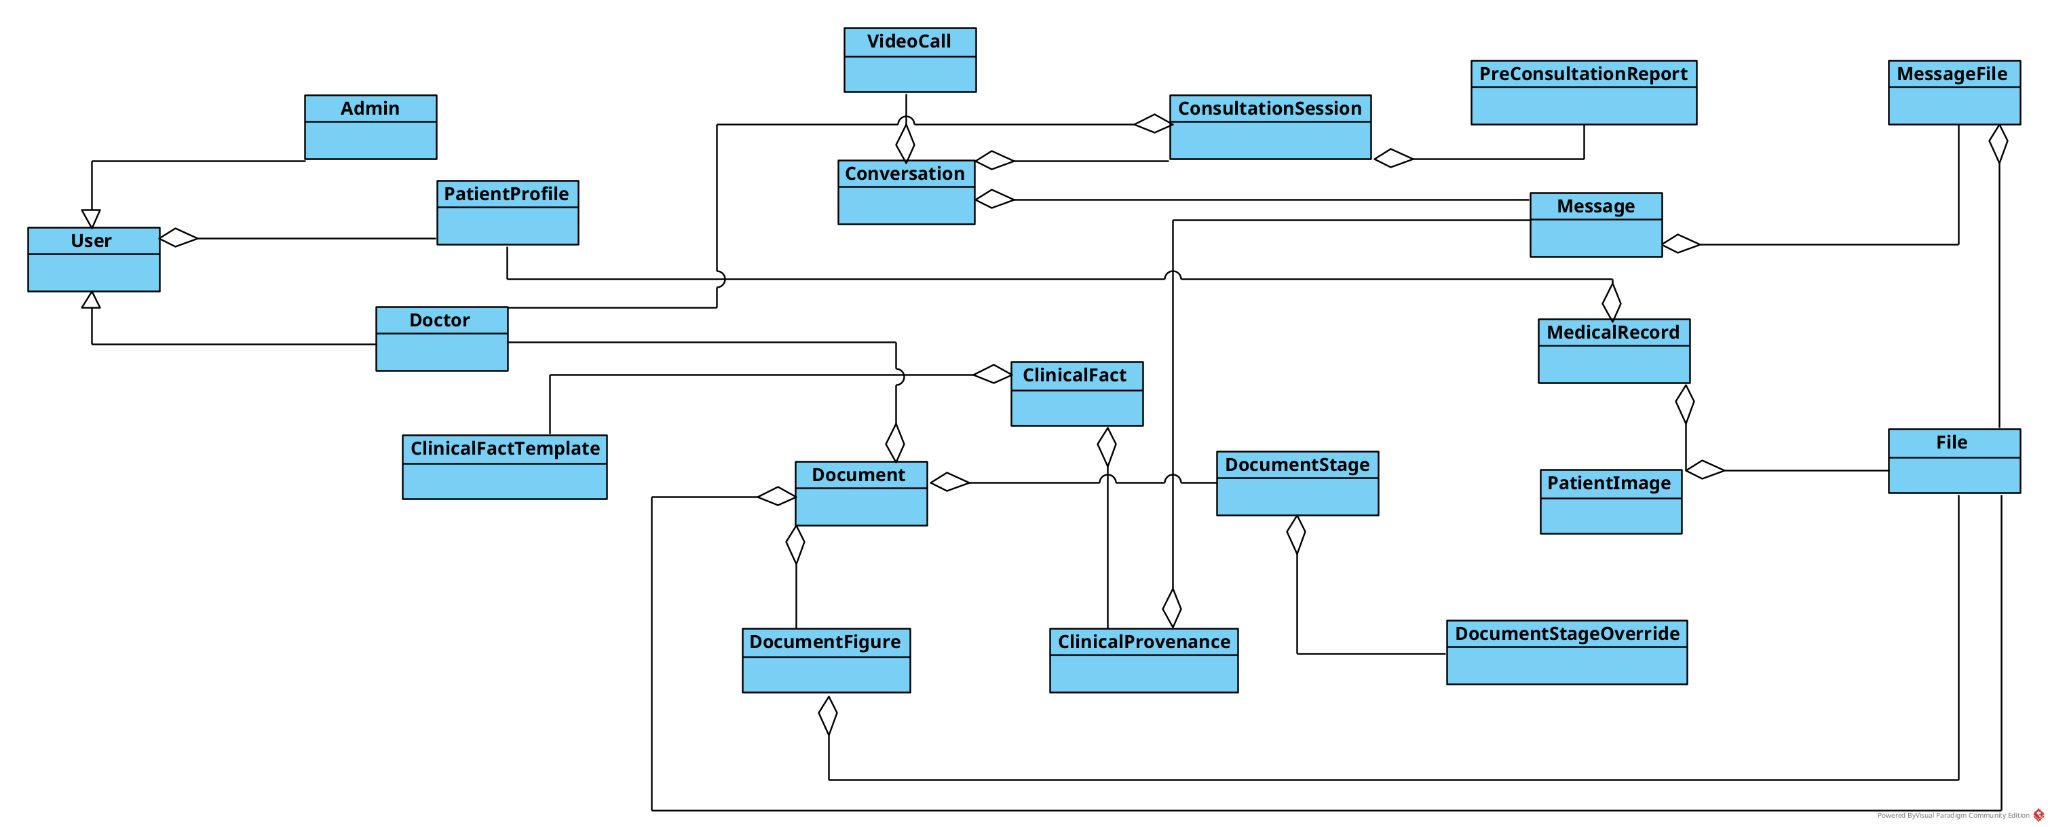
\includegraphics[width=0.95\linewidth]{chuong2/hinh/so_do_lop.png}
  \caption{Sơ đồ lớp thực thể của hệ thống}
  \label{fig:so_do_lop}
\end{sidewaysfigure}

Các lớp thực thể chính trong hệ thống được phân chia thành các nhóm miền nghiệp vụ rõ rệt:
\begin{itemize}
  \item \textbf{Nhóm Người dùng và Hồ sơ (\texttt{User}, \texttt{PatientProfile}, \texttt{Doctor}, \texttt{Admin}):} Quản lý tài khoản đăng nhập, thông tin chuyên môn của bác sĩ, và cho phép một tài khoản quản lý nhiều hồ sơ bệnh nhân (bản thân và các thành viên trong gia đình).
  \item \textbf{Nhóm Hội thoại và Tương tác (\texttt{Conversation}, \texttt{Message}, \texttt{MessageFile}, \texttt{VideoCall}):} Lưu trữ các phiên trao đổi tin nhắn giữa bệnh nhân, trợ lý AI và bác sĩ; ghi nhận các tập tin đính kèm và thông tin phiên gọi video trực tuyến.
  \item \textbf{Nhóm Lâm sàng và Bệnh án (\texttt{Episode}, \texttt{Appointment}, \texttt{Encounter}, \texttt{ClinicalFact}, \texttt{ClinicalProvenance}, \texttt{FinalizeReport}, \texttt{PatientImage}):} Quản lý đợt tiến triển bệnh (\textit{Episode}), lịch hẹn và lần khám, lưu vết nguồn gốc dữ kiện trích xuất từ tin nhắn (\textit{Provenance}), cùng báo cáo kết luận chẩn đoán và hình ảnh y khoa đã được bác sĩ xác nhận.
  \item \textbf{Nhóm Kho tri thức và Tài liệu (\texttt{Document}, \texttt{DocumentStage}, \texttt{DocumentOverride}, \texttt{File}):} Quản lý siêu dữ liệu tập tin lưu trữ trên MinIO, thông tin sách giáo trình y khoa, tiến trình thực thi qua từng bước của pipeline số hóa và các bản ghi can thiệp thủ công từ chuyên gia.
\end{itemize}

\subsection{Quan hệ giữa các lớp thực thể}

Mối quan hệ giữa các lớp thực thể trong hệ thống phản ánh chặt chẽ quy trình nghiệp vụ khám chữa bệnh và bảo đảm tính toàn vẹn dữ liệu:

\begin{itemize}
  \item \textbf{Quan hệ \texttt{User} -- \texttt{PatientProfile} (1--$n$):} Một tài khoản người dùng có thể tạo và quản lý nhiều hồ sơ bệnh nhân khác nhau. Mọi tương tác hội thoại, lịch hẹn và bệnh án lâm sàng đều liên kết trực tiếp với mã định danh \dbname{patient\_profile\_id} thay vì tài khoản \texttt{User}, giúp tách bạch lịch sử bệnh lý của từng cá nhân.
  \item \textbf{Quan hệ \texttt{Appointment} -- \texttt{Encounter} (1--1):} Bệnh nhân đặt lịch hẹn khám (\texttt{Appointment}) với một bác sĩ cụ thể. Khi bác sĩ tiếp nhận, một lần khám (\texttt{Encounter}) được khởi tạo để theo dõi tiến trình thăm khám thực tế. Mỗi lịch hẹn chỉ sinh ra một lần khám.
  \item \textbf{Quan hệ \texttt{Episode} -- \texttt{ClinicalFact} (1--$n$):} Một đợt bệnh biểu diễn một giai đoạn tổn thương da cụ thể, chứa nhiều dữ kiện lâm sàng (\texttt{ClinicalFact}). Dữ kiện dài hạn như tiền sử dị ứng, thuốc đang dùng được gắn với hồ sơ bệnh nhân và không thuộc đợt bệnh nào.
  \item \textbf{Quan hệ \texttt{ClinicalFact} -- \texttt{ClinicalProvenance} (1--$n$):} Mỗi dữ kiện lâm sàng có thể được ghi nhận từ nhiều nguồn khác nhau. Mỗi dòng lưu vết ghi lại một lần một nguồn (\texttt{chat}, \texttt{doctor}, \texttt{profile}) xác lập giá trị của dữ kiện, kèm trích dẫn nguyên văn và thời điểm ghi nhận.
  \item \textbf{Quan hệ \texttt{Message} -- \texttt{ClinicalProvenance} ($n$--1):} Mỗi dòng lưu vết trỏ tới tối đa một tin nhắn nguồn ở dịch vụ tư vấn, lưu dưới dạng id mềm và không ràng buộc khoá ngoại. Nhờ đó bác sĩ truy vết được dữ kiện do chatbot trích xuất về đúng tin nhắn và hình ảnh mà bệnh nhân đã gửi, phục vụ đối soát và kiểm chứng lâm sàng.
  \item \textbf{Quan hệ \texttt{Encounter} -- \texttt{FinalizeReport} (1--1):} Khi kết thúc lần khám, bác sĩ chốt báo cáo kết luận (\texttt{FinalizeReport}) gắn với \texttt{Encounter}. Báo cáo này lưu giữ snapshot toàn bộ nhận định chẩn đoán và dữ kiện lâm sàng đã được bác sĩ xác nhận. Nếu được đánh dấu là ca tham khảo chuẩn (\dbname{is\_reference\_case}), dữ liệu sẽ được ẩn danh và nạp sang kho tri thức vector (Qdrant) và đồ thị PJKG để phục vụ các ca tương tự sau này.
  \item \textbf{Quan hệ \texttt{Document} -- \texttt{DocumentStage} (1--$n$):} Một tài liệu giáo trình (\texttt{Document}) sở hữu nhiều bước xử lý (\texttt{DocumentStage}). Cặp \dbname{document\_id} và \dbname{stage\_id} là duy nhất, nên mỗi bước chỉ có một bản ghi trạng thái trên một tài liệu.
  \item \textbf{Quan hệ \texttt{DocumentStage} -- \texttt{DocumentOverride} (1--1):} Mỗi bước có tối đa một bản ghi \texttt{DocumentOverride} lưu các can thiệp chỉnh sửa tay của chuyên gia; khoá chính của bảng chính là \dbname{document\_stage\_id}. Nhờ vậy chạy lại máy không làm mất công sức hiệu đính của người duyệt.
\end{itemize}

\section{Thiết kế kiến trúc microservice}

\subsection{Phân rã service}

\subsubsection{Nguyên tắc phân rã}
Hệ thống được phân rã dựa trên nguyên lý thiết kế hướng miền (Domain-Driven Design - DDD). Mỗi dịch vụ chịu trách nhiệm cho một miền nghiệp vụ độc lập, sở hữu cơ sở dữ liệu riêng biệt (Database-per-Service) nhằm đảm bảo tính độc lập về triển khai, bảo trì và khả năng mở rộng quy mô linh hoạt theo nhu cầu tải.

\subsubsection{Danh sách service theo domain}
Dựa trên phân tích nghiệp vụ khám chữa bệnh da liễu và các tác vụ trí tuệ nhân tạo, hệ thống được phân chia thành 6 dịch vụ chính:
\begin{itemize}
  \item \dbname{gateway\_service}: API Gateway, quản lý định tuyến lưu lượng và reverse proxy.
  \item \dbname{identity\_service}: Quản lý tài khoản, phân quyền và hồ sơ bệnh nhân.
  \item \dbname{consultation\_service}: Quản lý phiên hội thoại, tin nhắn và kênh theo dõi sau khám.
  \item \dbname{clinical\_service}: Quản lý hồ sơ bệnh án, lịch hẹn, đợt bệnh và báo cáo kết luận.
  \item \dbname{knowledge\_service}: Quản lý pipeline số hóa sách, vector database và đồ thị tri thức.
  \item \dbname{ai\_service}: Quản lý tác nhân lập luận LangGraph, mô hình CNN và xử lý dữ kiện lâm sàng.
\end{itemize}

Mỗi dịch vụ sở hữu một lược đồ cơ sở dữ liệu riêng, không dùng chung bảng. Sơ đồ cơ sở dữ liệu của bốn dịch vụ có lưu trữ quan hệ được thể hiện trong Hình~\ref{fig:services_db}.

\begin{sidewaysfigure}[p]
  \centering
  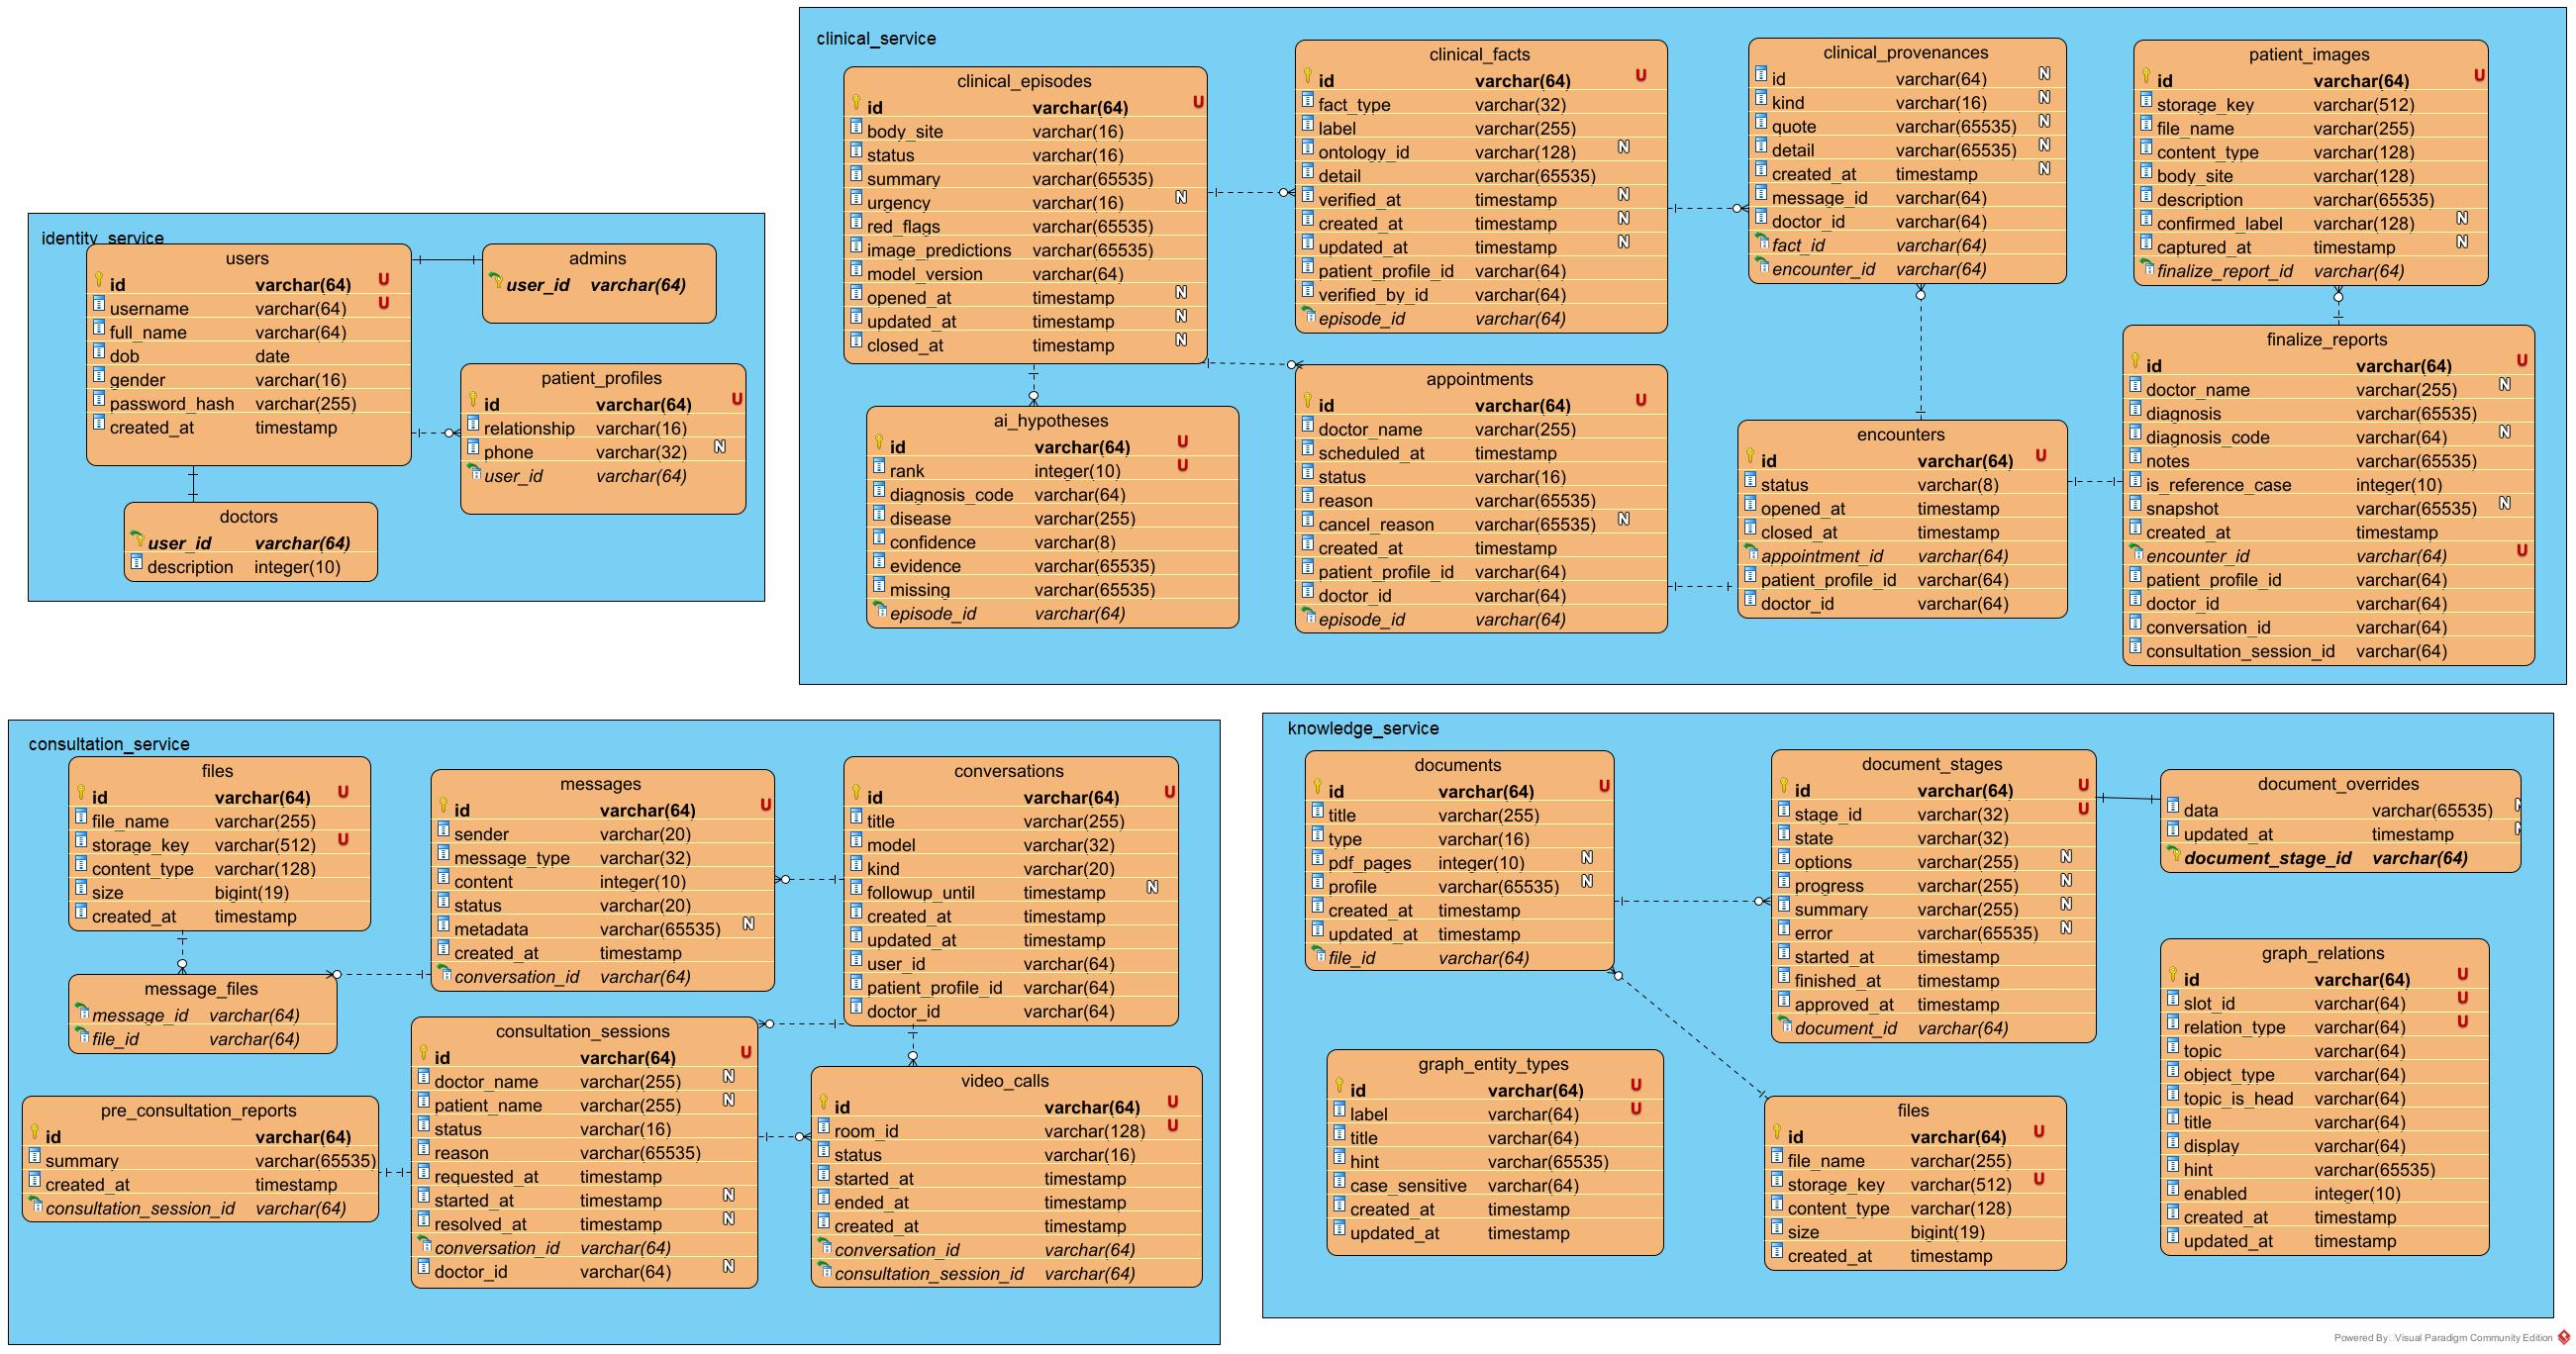
\includegraphics[width=0.95\linewidth]{chuong2/hinh/services_db.jpg}
  \caption{Sơ đồ cơ sở dữ liệu theo từng dịch vụ trong kiến trúc microservice}
  \label{fig:services_db}
\end{sidewaysfigure}
\clearpage

\subsubsection{Kiến trúc tổng thể (Client, API Gateway, Server, Database)}
Kiến trúc tổng thể của hệ thống gồm tầng Client (giao diện Next.js cho Bệnh nhân, Bác sĩ và Quản trị viên), tầng cổng kết nối API Gateway tiếp nhận các yêu cầu REST/SSE, tầng dịch vụ nghiệp vụ (Spring Boot và Python FastAPI/LangGraph) cùng tầng lưu trữ dữ liệu đa mô hình gồm PostgreSQL, Redis, MinIO, Qdrant và Neo4j. Bốn tầng này được thể hiện trong Hình~\ref{fig:kien_truc_tong_the}.

\begin{figure}[H]
  \centering
  \begin{singlespace}
  \begin{tikzpicture}[
    font=\scriptsize,
    >=Stealth,
    tierbox/.style={rounded corners=2pt, align=center, inner sep=2pt, line width=1.3pt},
    svc/.style={draw=teal!90!black, fill=teal!4, rounded corners=2pt, align=center,
      minimum width=3.0cm, minimum height=0.8cm, inner sep=2pt, line width=1.1pt},
    data/.style={draw=green!50!black, fill=green!7, rounded corners=2pt, align=center,
      minimum height=1.6cm, inner sep=1pt, line width=1.1pt},
    infra/.style={draw=black!60, fill=black!5, rounded corners=2pt, align=center,
      minimum height=1.6cm, inner sep=1pt, line width=1pt},
    frame/.style={draw=black!60, fill=black!3, rounded corners=3pt, line width=0.9pt},
    link/.style={->, draw=black!85, line width=0.8pt},
    external/.style={draw=black!70, dashed, fill=black!3, rounded corners=2pt, align=center,
      inner sep=2pt, line width=1pt},
    note/.style={font=\scriptsize, text=black!80, align=center}
  ]

  % ---------- tầng client ----------
  \node[tierbox, draw=blue!75!black, fill=blue!4, minimum width=6.0cm, minimum height=0.8cm] (client) at (8.0,14.5)
    {\textbf{Next.js}};

  % ---------- tầng gateway ----------
  \node[tierbox, draw=red!70!black, fill=red!4, minimum width=15.7cm, minimum height=0.8cm] (gateway) at (8.0,13.15)
    {\textbf{gateway-service} (Spring Cloud Gateway)};

  % ---------- tầng dịch vụ ----------
  \draw[frame] (0.05,11.0) rectangle (15.95,12.4);

  \node[svc] (identity) at (1.7,11.7) {\textbf{identity-service}};
  \node[svc] (consultation) at (4.85,11.7) {\textbf{consultation-service}};
  \node[svc] (clinical) at (8.0,11.7) {\textbf{clinical-service}};
  \node[svc] (knowledge) at (11.15,11.7) {\textbf{knowledge-service}};
  \node[svc] (ai) at (14.3,11.7) {\textbf{ai-service}};

  % ---------- mô hình ngôn ngữ ngoài hệ thống ----------
  \node[external, minimum width=3.2cm, minimum height=0.8cm] (llm) at (14.3,10.05)
    {\textbf{LLM}\\\\{\scriptsize OpenRouter · Ollama}};

  % ---------- tầng dữ liệu ----------
  \draw[frame] (0.05,6.3) rectangle (15.95,9.05);
  \node[note, anchor=west] at (0.3,8.82) {mỗi dịch vụ sở hữu một database riêng};

  \node[data, minimum width=3.8cm] (postgres) at (2.3,7.5)
    {\textbf{PostgreSQL}\\{\scriptsize identity · consultation}\\{\scriptsize clinical · knowledge}\\{\scriptsize ai (checkpoint)}};
  \node[infra, minimum width=2.1cm] (redis) at (5.43,7.5)
    {\textbf{Redis}\\{\scriptsize token, stream}};
  \node[infra, minimum width=2.1cm] (minio) at (7.71,7.5)
    {\textbf{MinIO}\\{\scriptsize ảnh, PDF}};
  \node[infra, minimum width=2.1cm] (qdrant) at (9.99,7.5)
    {\textbf{Qdrant}\\{\scriptsize vector}};
  \node[infra, minimum width=2.1cm] (neo4j) at (12.27,7.5)
    {\textbf{Neo4j}\\{\scriptsize đồ thị}};
  \node[infra, minimum width=2.1cm] (rabbit) at (14.55,7.5)
    {\textbf{RabbitMQ}\\{\scriptsize pipeline sách}};

  % ---------- liên kết ----------
  \draw[link] (client.south) -- (gateway.north)
    node[midway, right=3pt, note] {HTTPS: REST \texttt{/api/v1/**}, SSE};
  \foreach \s in {identity, consultation, clinical, knowledge}
    \draw[link] (\s.north|-gateway.south) -- (\s.north);
  \draw[link] (8.0,11.0) -- (8.0,9.05)
    node[midway, left=3pt, note] {SQL · Redis · S3 · vector · graph};
  \draw[link, dashed] (ai.south) -- (llm.north)
    node[pos=0.58, right=3pt, note] {gọi LLM};

\end{tikzpicture}
  \end{singlespace}
  \caption{Kiến trúc tổng thể của hệ thống theo bốn tầng: client, API Gateway, dịch vụ nghiệp vụ và lưu trữ dữ liệu}
  \label{fig:kien_truc_tong_the}
\end{figure}


\subsubsection{Giao tiếp giữa các dịch vụ}
Các dịch vụ nghiệp vụ trao đổi nội bộ thông qua hai cơ chế chính:
\begin{itemize}
  \item \textbf{REST API nội bộ (\texttt{/internal/...}):} Sử dụng giao thức HTTP/1.1 kèm khóa xác thực bí mật chung (\texttt{X-Internal-Key}) để thực hiện các lời gọi đồng bộ giữa các service.
  \item \textbf{Redis Stream:} Sử dụng kênh stream \texttt{conversation:events:\{id\}} để phát và phát lại (replay) các sự kiện xử lý thời gian thực từ Agent đến Client thông qua Server-Sent Events (SSE).
\end{itemize}

\subsection{Thiết kế dịch vụ API Gateway (\dbname{gateway\_service})}

\subsubsection{Chức năng và cơ chế định tuyến}
Dịch vụ API Gateway được xây dựng trên nền tảng Spring Cloud Gateway, đóng vai trò là điểm truy cập duy nhất (Single Point of Entry) cho toàn bộ các ứng dụng Client bên ngoài. Gateway thực hiện định tuyến động các yêu cầu dựa trên tiền tố đường dẫn (Path Prefix) tới các dịch vụ nghiệp vụ tương ứng ở phía sau.

\subsubsection{Cấu hình triển khai}
Gateway lắng nghe tại cổng \texttt{3040}, thiết lập cấu hình CORS tập trung, chuyển tiếp nguyên vẹn các luồng dữ liệu streaming (SSE) và quản lý chuyển tiếp các header xác thực mà không can thiệp sâu vào xử lý nghiệp vụ nội bộ.

\subsection{Thiết kế dịch vụ định danh (\dbname{identity\_service})}

\subsubsection{Chức năng và giao diện lập trình (API)}
Dịch vụ đảm nhận đăng ký, xác thực danh tính người dùng bằng JSON Web Token (JWT), quản lý cơ chế xoay vòng Refresh Token trên Redis, và quản lý hồ sơ thông tin của các bác sĩ cũng như hồ sơ bệnh nhân cá nhân/gia đình.

\subsubsection{Thiết kế cơ sở dữ liệu}
Dịch vụ quản trị cơ sở dữ liệu PostgreSQL độc lập (\dbname{identity\_db}) gồm tài khoản, vai trò và hồ sơ bệnh nhân.
\begin{itemize}
\raggedright
  \item \textbf{Danh sách các bảng:}
  \begin{itemize}
    \item \dbname{users}: \dbname{id} (PK), \dbname{username} (UQ), \dbname{full\_name}, \dbname{dob}, \dbname{gender}, \dbname{password\_hash}, \dbname{created\_at}.
    \item \dbname{doctors}: \dbname{user\_id} \mbox{(PK, FK $\rightarrow$ \dbname{users.id})}, \dbname{description}.
    \item \dbname{admins}: \dbname{user\_id} \mbox{(PK, FK $\rightarrow$ \dbname{users.id})}.
    \item \dbname{patient\_profiles}: \dbname{id} (PK), \dbname{user\_id} \mbox{(FK $\rightarrow$ \dbname{users.id})}, \dbname{full\_name}, \dbname{dob}, \dbname{gender}, \dbname{relationship}, \dbname{phone}, \dbname{created\_at}.
  \end{itemize}
  \item \textbf{Quan hệ giữa các bảng:}
  \begin{itemize}
    \item \dbname{users} -- \dbname{doctors}: Quan hệ 1--1.
    \item \dbname{users} -- \dbname{admins}: Quan hệ 1--1.
    \item \dbname{users} -- \dbname{patient\_profiles}: Quan hệ 1--$n$.
  \end{itemize}
\end{itemize}

\begin{figure}[H]
  \centering
  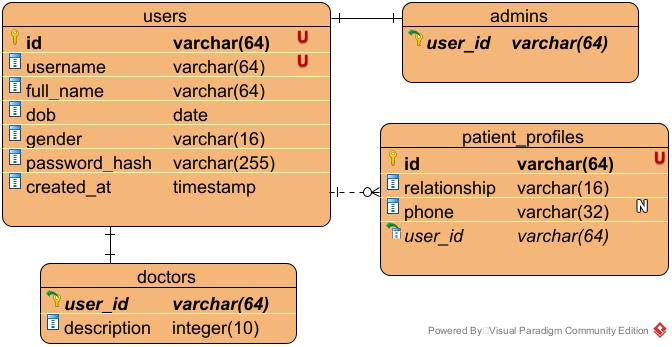
\includegraphics[width=0.95\linewidth,height=0.7\textheight,keepaspectratio]{chuong2/hinh/identity_db.jpg}
  \caption{Sơ đồ cơ sở dữ liệu dịch vụ định danh}
  \label{fig:db_identity}
\end{figure}

\subsection{Thiết kế dịch vụ tư vấn (\dbname{consultation\_service})}

\subsubsection{Chức năng và giao diện lập trình (API)}
Dịch vụ chịu trách nhiệm khởi tạo và lưu trữ các cuộc hội thoại (\texttt{Conversation}), điều phối tin nhắn gửi đến tác nhân AI hoặc bác sĩ, quản lý kênh theo dõi sau khám (\texttt{FollowupChannel}) và xử lý tín hiệu kết nối cho các cuộc gọi video trực tuyến (\texttt{VideoCall}).

\subsubsection{Thiết kế cơ sở dữ liệu}
Dịch vụ sở hữu cơ sở dữ liệu PostgreSQL (\dbname{consultation\_db}) cho hội thoại, tin nhắn, phiên tư vấn và cuộc gọi video; sự kiện thời gian thực đi qua Redis Stream.
\begin{itemize}
\raggedright
  \item \textbf{Danh sách các bảng:}
  \begin{itemize}
    \item \dbname{files}: \dbname{id} (PK), \dbname{file\_name}, \dbname{storage\_key} (UQ), \dbname{content\_type}, \dbname{size}, \dbname{created\_at}.
    \item \dbname{conversations}: \dbname{id} (PK), \dbname{user\_id}, \dbname{patient\_profile\_id}, \dbname{title}, \dbname{model}, \dbname{kind}, \dbname{encounter\_id} (UQ), \dbname{doctor\_id}, \dbname{followup\_until}, \dbname{created\_at}, \dbname{updated\_at}.
    \item \dbname{consultation\_sessions}: \dbname{id} (PK), \dbname{conversation\_id} \mbox{(FK $\rightarrow$ \dbname{conversations.id})}, \dbname{doctor\_id}, \dbname{doctor\_name}, \dbname{patient\_name}, \dbname{status}, \dbname{reason}, \dbname{requested\_at}, \dbname{started\_at}, \dbname{resolved\_at}.
    \item \dbname{messages}: \dbname{id} (PK), \dbname{conversation\_id} \mbox{(FK $\rightarrow$ \dbname{conversations.id})}, \dbname{sender}, \dbname{message\_type}, \dbname{video\_call\_id} \mbox{(FK $\rightarrow$ \dbname{video\_calls.id})}, \dbname{consultation\_session\_id} \mbox{(FK $\rightarrow$ \dbname{consultation\_sessions.id})}, \dbname{content}, \dbname{status}, \dbname{metadata}, \dbname{created\_at}.
    \item \dbname{video\_calls}: \dbname{id} (PK), \dbname{conversation\_id} \mbox{(FK $\rightarrow$ \dbname{conversations.id})}, \dbname{consultation\_session\_id} \mbox{(FK $\rightarrow$ \dbname{consultation\_sessions.id})}, \dbname{room\_id} (UQ), \dbname{status}, \dbname{started\_at}, \dbname{ended\_at}, \dbname{created\_at}.
    \item \dbname{message\_files}: \dbname{message\_id} \mbox{(PK, FK $\rightarrow$ \dbname{messages.id})}, \dbname{file\_id} \mbox{(PK, FK $\rightarrow$ \dbname{files.id})}.
    \item \dbname{pre\_consultation\_reports}: \dbname{id} (PK), \dbname{consultation\_session\_id} \mbox{(UQ, FK $\rightarrow$ \dbname{consultation\_sessions.id})}, \dbname{summary}, \dbname{created\_at}.
  \end{itemize}
  \item \textbf{Quan hệ giữa các bảng:}
  \begin{itemize}
    \item \dbname{conversations} -- \dbname{consultation\_sessions}: Quan hệ 1--$n$.
    \item \dbname{conversations} -- \dbname{messages}: Quan hệ 1--$n$.
    \item \dbname{conversations} -- \dbname{video\_calls}: Quan hệ 1--$n$.
    \item \dbname{consultation\_sessions} -- \dbname{video\_calls}: Quan hệ 1--$n$.
    \item \dbname{consultation\_sessions} -- \dbname{messages}: Quan hệ 1--$n$.
    \item \dbname{consultation\_sessions} -- \dbname{pre\_consultation\_reports}: Quan hệ 1--1.
    \item \dbname{video\_calls} -- \dbname{messages}: Quan hệ 1--$n$.
    \item \dbname{messages} -- \dbname{message\_files}: Quan hệ 1--$n$.
    \item \dbname{files} -- \dbname{message\_files}: Quan hệ 1--$n$.
  \end{itemize}
\end{itemize}

\begin{figure}[H]
  \centering
  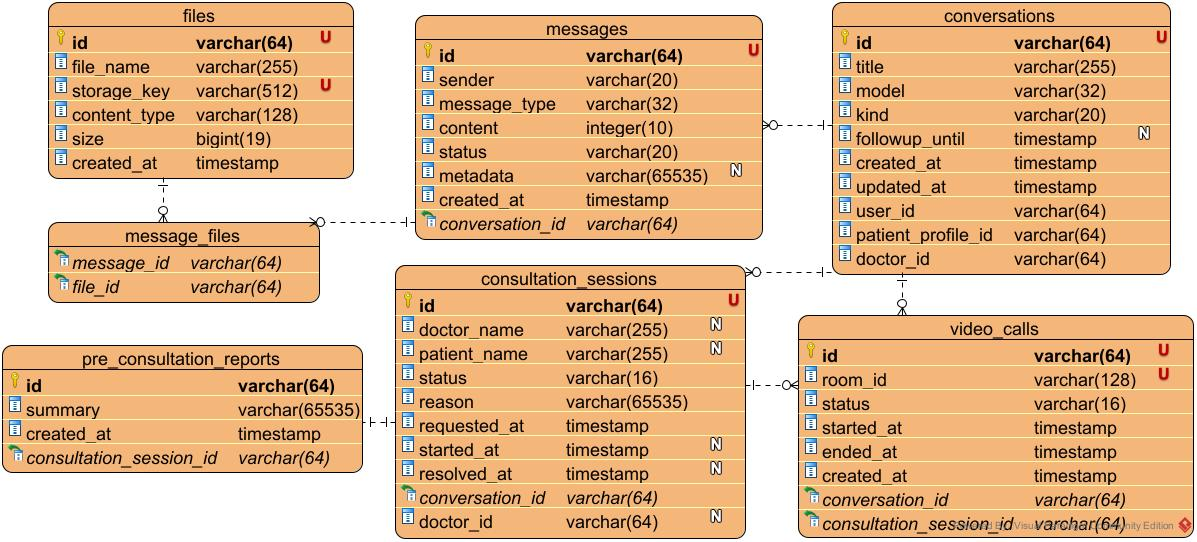
\includegraphics[width=0.95\linewidth,height=0.7\textheight,keepaspectratio]{chuong2/hinh/consultation_db.jpg}
  \caption{Sơ đồ cơ sở dữ liệu dịch vụ tư vấn}
  \label{fig:db_consultation}
\end{figure}

\subsection{Thiết kế dịch vụ lâm sàng (\dbname{clinical\_service})}

\subsubsection{Chức năng và giao diện lập trình (API)}
Dịch vụ quản lý toàn bộ vòng đời bệnh lý của bệnh nhân: lập lịch hẹn khám (\texttt{Appointment}), tiếp nhận lần khám (\texttt{Encounter}), theo dõi đợt bệnh (\texttt{Episode}), lưu trữ các dữ kiện lâm sàng (\texttt{ClinicalFact}) và chốt báo cáo kết luận khám bệnh (\texttt{FinalizeReport}).

\subsubsection{Thiết kế cơ sở dữ liệu}
Dịch vụ quản trị cơ sở dữ liệu \dbname{clinical\_db} cho đợt bệnh, dữ kiện lâm sàng, lịch hẹn, lần khám và báo cáo kết luận.
\begin{itemize}
\raggedright
  \item \textbf{Danh sách các bảng:}
  \begin{itemize}
    \item \dbname{clinical\_episodes}: \dbname{id} (PK), \dbname{patient\_profile\_id}, \dbname{body\_site}, \dbname{status}, \dbname{last\_conversation\_id}, \dbname{summary}, \dbname{summary\_at}, \dbname{urgency}, \dbname{red\_flags}, \dbname{image\_predictions}, \dbname{model\_version}, \dbname{opened\_at}, \dbname{updated\_at}, \dbname{closed\_at}.
    \item \dbname{ai\_hypotheses}: \dbname{id} (PK), \dbname{episode\_id} \mbox{(FK $\rightarrow$ \dbname{clinical\_episodes.id})}, \dbname{rank}, \dbname{diagnosis\_code}, \dbname{disease}, \dbname{confidence}, \dbname{evidence}, \dbname{missing}. UQ (\dbname{episode\_id}, \dbname{rank}).
    \item \dbname{clinical\_facts}: \dbname{id} (PK), \dbname{patient\_profile\_id}, \dbname{episode\_id} \mbox{(FK $\rightarrow$ \dbname{clinical\_episodes.id})}, \dbname{fact\_type}, \dbname{label}, \dbname{ontology\_id}, \dbname{detail}, \dbname{verified\_at}, \dbname{verified\_by\_id}, \dbname{created\_at}, \dbname{updated\_at}.
    \item \dbname{appointments}: \dbname{id} (PK), \dbname{patient\_profile\_id}, \dbname{episode\_id} \mbox{(FK $\rightarrow$ \dbname{clinical\_episodes.id})}, \dbname{doctor\_id}, \dbname{doctor\_name}, \dbname{scheduled\_at}, \dbname{status}, \dbname{reason}, \dbname{cancel\_reason}, \dbname{created\_at}.
    \item \dbname{encounters}: \dbname{id} (PK), \dbname{appointment\_id} \mbox{(UQ, FK $\rightarrow$ \dbname{appointments.id})}, \dbname{patient\_profile\_id}, \dbname{doctor\_id}, \dbname{status}, \dbname{opened\_at}, \dbname{closed\_at}.
    \item \dbname{clinical\_provenances}: \dbname{id} (PK), \dbname{fact\_id} \mbox{(FK $\rightarrow$ \dbname{clinical\_facts.id})}, \dbname{kind}, \dbname{message\_id}, \dbname{quote}, \dbname{doctor\_id}, \dbname{encounter\_id} \mbox{(FK $\rightarrow$ \dbname{encounters.id})}, \dbname{detail}, \dbname{created\_at}.
    \item \dbname{finalize\_reports}: \dbname{id} (PK), \dbname{patient\_profile\_id}, \dbname{doctor\_id}, \dbname{doctor\_name}, \dbname{diagnosis}, \dbname{notes}, \dbname{is\_reference\_case}, \dbname{consultation\_session\_id} (UQ), \dbname{conversation\_id}, \dbname{encounter\_id} \mbox{(UQ, FK $\rightarrow$ \dbname{encounters.id})}, \dbname{diagnosis\_code}, \dbname{snapshot}, \dbname{created\_at}.
    \item \dbname{patient\_images}: \dbname{id} (PK), \dbname{finalize\_report\_id} \mbox{(FK $\rightarrow$ \dbname{finalize\_reports.id})}, \dbname{storage\_key}, \dbname{file\_name}, \dbname{content\_type}, \dbname{body\_site}, \dbname{description}, \dbname{confirmed\_label}, \dbname{captured\_at}.
  \end{itemize}
  \item \textbf{Quan hệ giữa các bảng:}
  \begin{itemize}
    \item \dbname{clinical\_episodes} -- \dbname{ai\_hypotheses}: Quan hệ 1--$n$.
    \item \dbname{clinical\_episodes} -- \dbname{clinical\_facts}: Quan hệ 1--$n$.
    \item \dbname{clinical\_episodes} -- \dbname{appointments}: Quan hệ 1--$n$.
    \item \dbname{appointments} -- \dbname{encounters}: Quan hệ 1--1.
    \item \dbname{clinical\_facts} -- \dbname{clinical\_provenances}: Quan hệ 1--$n$.
    \item \dbname{encounters} -- \dbname{clinical\_provenances}: Quan hệ 1--$n$.
    \item \dbname{encounters} -- \dbname{finalize\_reports}: Quan hệ 1--1.
    \item \dbname{finalize\_reports} -- \dbname{patient\_images}: Quan hệ 1--$n$.
  \end{itemize}
\end{itemize}
Ngoài khoá chính và khoá ngoại, \dbname{clinical\_db} còn dùng ba chỉ mục duy nhất có điều kiện: mỗi vùng cơ thể chỉ có một đợt đang mở, mỗi đợt chỉ có một lịch hẹn còn hiệu lực, và mỗi cặp (phạm vi, loại, nhãn) dữ kiện chỉ có một dòng.

\begin{figure}[H]
  \centering
  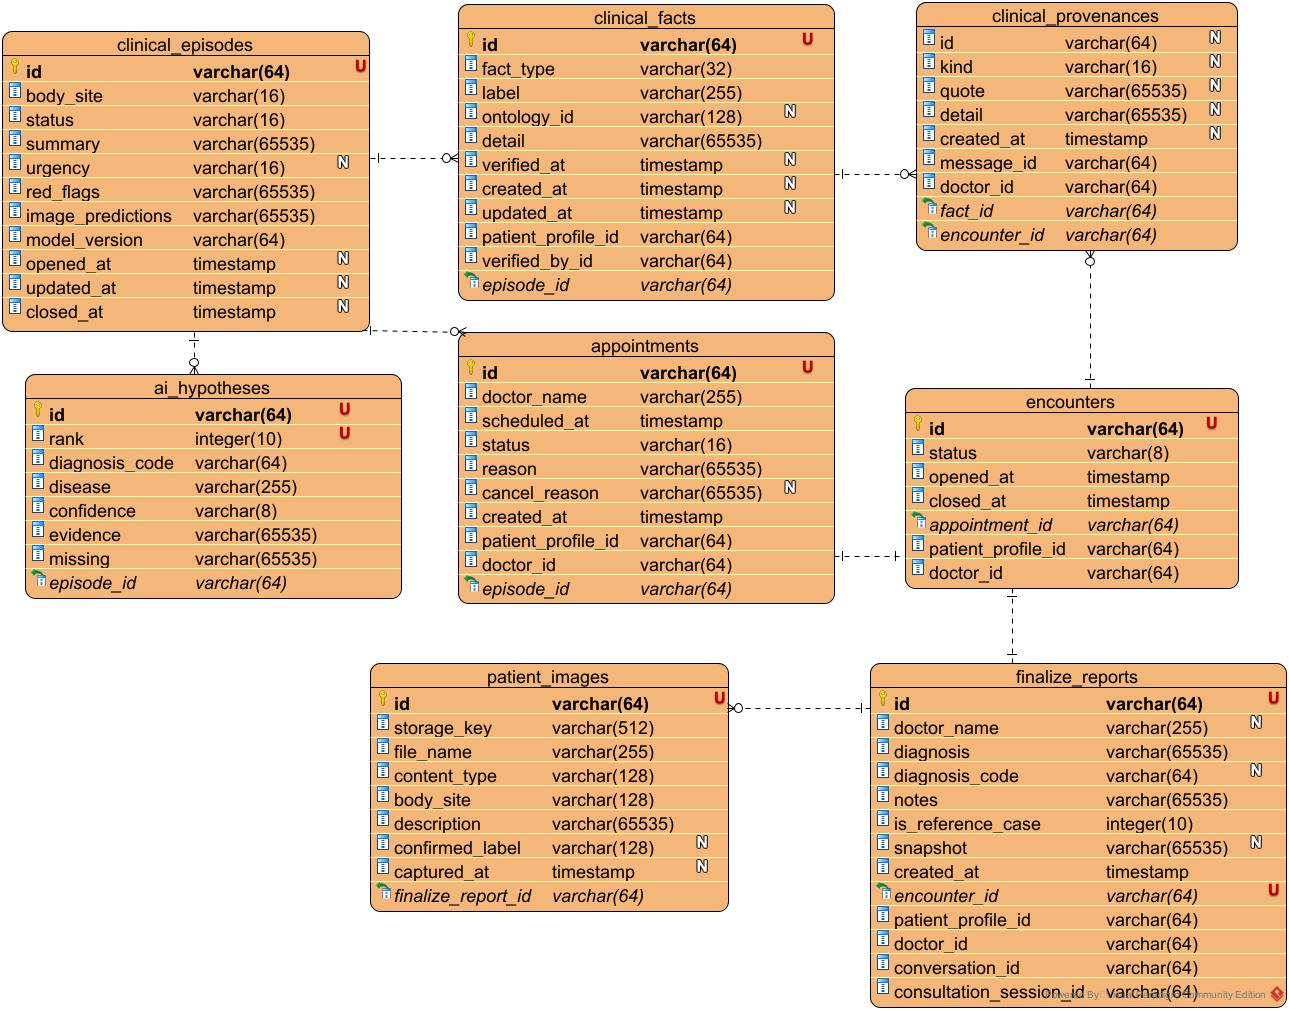
\includegraphics[width=0.95\linewidth,height=0.7\textheight,keepaspectratio]{chuong2/hinh/clinical_db.jpg}
  \caption{Sơ đồ cơ sở dữ liệu dịch vụ lâm sàng}
  \label{fig:db_clinical}
\end{figure}

\subsection{Thiết kế dịch vụ tri thức y khoa (\dbname{knowledge\_service})}

\subsubsection{Chức năng và giao diện lập trình (API)}
Dịch vụ cung cấp các API phục vụ pipeline số hóa tài liệu giáo trình da liễu, tra cứu ngữ nghĩa đa phương thức (Hybrid Search kết hợp Dense Vector và BM25 Sparse), truy vấn đồ thị tri thức bệnh nhân Neo4j và cung cấp URL trích dẫn trang sách y khoa có thể đối soát trực tiếp.

\subsubsection{Thiết kế cơ sở dữ liệu và kho tri thức}
Dịch vụ lưu siêu dữ liệu tài liệu, tiến trình pipeline và danh mục đồ thị trong PostgreSQL (\dbname{knowledge\_db}); nội dung vector ở Qdrant, đồ thị tri thức ở Neo4j, tệp gốc ở MinIO.
\begin{itemize}
\raggedright
  \item \textbf{Danh sách các bảng:}
  \begin{itemize}
    \item \dbname{files}: \dbname{id} (PK), \dbname{file\_name}, \dbname{storage\_key} (UQ), \dbname{content\_type}, \dbname{size}, \dbname{created\_at}.
    \item \dbname{documents}: \dbname{id} (PK), \dbname{title}, \dbname{type}, \dbname{source\_file\_id} \mbox{(FK $\rightarrow$ \dbname{files.id})}, \dbname{ingested\_file\_id} \mbox{(FK $\rightarrow$ \dbname{files.id})}, \dbname{pdf\_pages}, \dbname{uploaded\_by\_id}, \dbname{profile}, \dbname{created\_at}, \dbname{updated\_at}.
    \item \dbname{document\_stages}: \dbname{id} (PK), \dbname{document\_id} \mbox{(FK $\rightarrow$ \dbname{documents.id})}, \dbname{stage\_id}, \dbname{state}, \dbname{options}, \dbname{progress}, \dbname{summary}, \dbname{error}, \dbname{started\_at}, \dbname{finished\_at}, \dbname{approved\_at}. UQ (\dbname{document\_id}, \dbname{stage\_id}).
    \item \dbname{document\_overrides}: \dbname{document\_stage\_id} \mbox{(PK, FK $\rightarrow$ \dbname{document\_stages.id})}, \dbname{data}, \dbname{updated\_at}.
    \item \dbname{graph\_entity\_types}: \dbname{id} (PK), \dbname{label} (UQ), \dbname{title}, \dbname{hint}, \dbname{case\_sensitive}, \dbname{created\_at}, \dbname{updated\_at}.
    \item \dbname{graph\_relations}: \dbname{id} (PK), \dbname{slot\_id} (UQ), \dbname{relation\_type} (UQ), \dbname{topic}, \dbname{object\_type}, \dbname{topic\_is\_head}, \dbname{title}, \dbname{display}, \dbname{hint}, \dbname{entity\_hint}, \dbname{enabled}, \dbname{created\_at}, \dbname{updated\_at}.
  \end{itemize}
  \item \textbf{Quan hệ giữa các bảng:}
  \begin{itemize}
    \item \dbname{files} -- \dbname{documents}: Quan hệ 1--$n$.
    \item \dbname{documents} -- \dbname{document\_stages}: Quan hệ 1--$n$.
    \item \dbname{document\_stages} -- \dbname{document\_overrides}: Quan hệ 1--1.
  \end{itemize}
\end{itemize}

\begin{figure}[H]
  \centering
  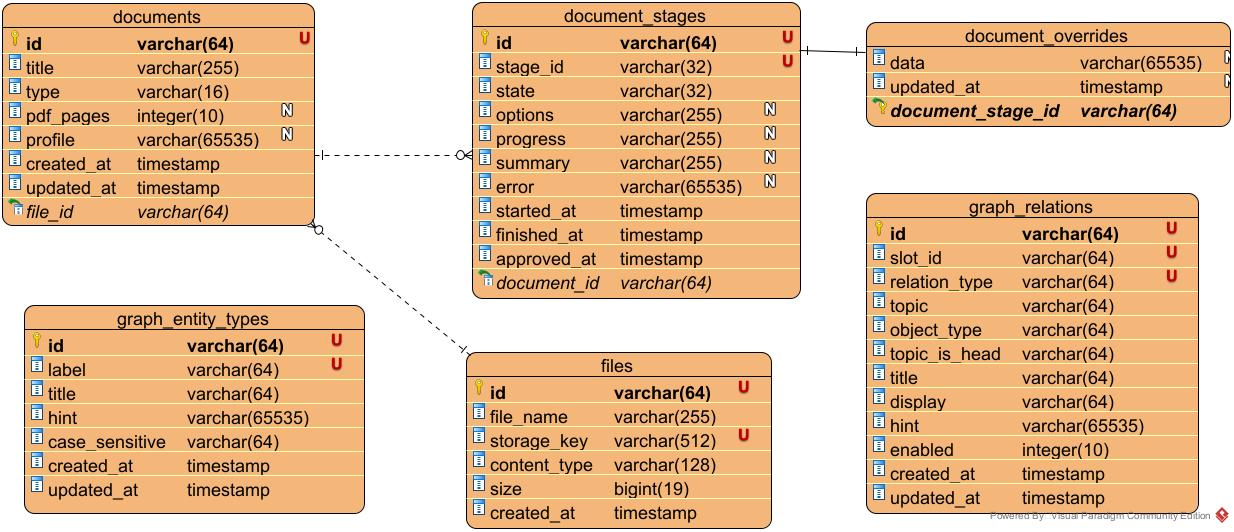
\includegraphics[width=0.95\linewidth,height=0.7\textheight,keepaspectratio]{chuong2/hinh/knowledge_db.jpg}
  \caption{Sơ đồ cơ sở dữ liệu dịch vụ tri thức y khoa}
  \label{fig:db_knowledge}
\end{figure}

\subsection{Thiết kế dịch vụ trí tuệ nhân tạo (\dbname{ai\_service})}

\subsubsection{Chức năng và giao diện lập trình (API)}
Dịch vụ tiếp nhận lượt tương tác qua API nội bộ \texttt{POST /internal/turns}, kích hoạt đồ thị lập luận LangGraph để truy xuất tri thức và sinh lời thoại tư vấn, gọi mô hình phân loại ảnh CNN, và trích xuất tự động các dữ kiện lâm sàng từ mô tả của bác sĩ khi chốt hồ sơ.

\subsubsection{Kiến trúc tác nhân và mô hình AI}
Dịch vụ tích hợp mô hình phân loại đa tổn thương Multi-scale Adaptive CNN với mô hình ngôn ngữ lớn (LLM) theo mô hình tác nhân ReAct có bộ nhớ ngữ cảnh và khả năng tự động gọi công cụ tra cứu tri thức chuyên sâu.

\subsubsection{Thiết kế lưu trữ trạng thái}
Dịch vụ giữ checkpoint của đồ thị lập luận và bộ nhớ dài hạn của tác nhân trong database \texttt{ai}, schema \texttt{langgraph}. Các bảng do thư viện LangGraph tự tạo khi khởi động, không có khoá ngoại sang dữ liệu nghiệp vụ.
\begin{itemize}
\raggedright
  \item \textbf{Danh sách các bảng:}
  \begin{itemize}
    \item \dbname{checkpoints}: \dbname{thread\_id} (PK), \dbname{checkpoint\_ns} (PK), \dbname{checkpoint\_id} (PK), \dbname{parent\_checkpoint\_id}, \dbname{type}, \dbname{checkpoint}, \dbname{metadata}.
    \item \dbname{checkpoint\_blobs}: \dbname{thread\_id} (PK), \dbname{checkpoint\_ns} (PK), \dbname{channel} (PK), \dbname{version} (PK), \dbname{type}, \dbname{blob}.
    \item \dbname{checkpoint\_writes}: \dbname{thread\_id} (PK), \dbname{checkpoint\_ns} (PK), \dbname{checkpoint\_id} (PK), \dbname{task\_id} (PK), \dbname{idx} (PK), \dbname{channel}, \dbname{type}, \dbname{blob}, \dbname{task\_path}.
    \item \dbname{store}: \dbname{prefix} (PK), \dbname{key} (PK), \dbname{value}, \dbname{created\_at}, \dbname{updated\_at}, \dbname{expires\_at}.
    \item \dbname{checkpoint\_migrations}, \dbname{store\_migrations}: phiên bản schema do thư viện quản lý.
  \end{itemize}
  \item \textbf{Quan hệ giữa các bảng:}
  \begin{itemize}
    \item \dbname{checkpoints} -- \dbname{checkpoint\_blobs}: Quan hệ 1--$n$.
    \item \dbname{checkpoints} -- \dbname{checkpoint\_writes}: Quan hệ 1--$n$.
  \end{itemize}
\end{itemize}

\section{Luồng xử lý các chức năng chính}

\subsection{Đăng nhập và đăng ký}

\subsubsection{Mô tả luồng}
Người dùng gửi thông tin đăng ký hoặc đăng nhập thông qua API Gateway. Dịch vụ \dbname{identity\_service} tiến hành xác thực mật khẩu (được mã hóa bằng bcrypt), phát hành cặp token (Access Token và Refresh Token) và trả về cho Client.

\subsubsection{Biểu đồ tuần tự}
Tiến trình tương tác giữa Client, API Gateway và \dbname{identity\_service} trong quá trình xác thực và cấp phát mã định danh được mô hình hóa nhằm đảm bảo an toàn truy cập trên toàn hệ thống.

\subsection{Hỏi đáp với chatbot tiền chẩn đoán}

\subsubsection{Mô tả luồng}
Bệnh nhân gửi tin nhắn kèm hình ảnh tổn thương da. \dbname{consultation\_service} lưu trữ tin nhắn và gửi yêu cầu lượt chạy sang \dbname{ai\_service}. Tác nhân AI gọi mô hình CNN để dự đoán nhãn tổn thương, gọi \dbname{knowledge\_service} để tra cứu tài liệu và stream câu trả lời về cho bệnh nhân qua Redis Stream và SSE. Kết thúc lượt, AI tự động ghi nhận các dữ kiện lâm sàng sang \dbname{clinical\_service}.

\subsubsection{Biểu đồ tuần tự}
Biểu đồ tuần tự minh họa luồng trao đổi bất đồng bộ giữa Client, Gateway, Consultation Service, AI Service, Knowledge Service và Clinical Service trong một lượt tư vấn hoàn chỉnh.

\subsection{Đặt lịch hẹn và tiếp nhận lần khám}

\subsubsection{Mô tả luồng}
Bệnh nhân chọn bác sĩ và thời gian khám trên giao diện để tạo lịch hẹn (\texttt{Appointment}). Bác sĩ kiểm tra danh sách ca và tiếp nhận lần khám (\texttt{Encounter}), hệ thống tự động tải dữ liệu tổng hợp tiền khám từ chatbot để bác sĩ chuẩn bị trước buổi thăm khám.

\subsubsection{Biểu đồ tuần tự}
Mô hình hóa chuỗi tương tác đặt lịch và khởi tạo lần khám giữa bệnh nhân, bác sĩ và dịch vụ lâm sàng.

\subsection{Tư vấn trực tiếp và gọi video với bác sĩ}

\subsubsection{Mô tả luồng}
Trong quá trình khám, bác sĩ và bệnh nhân trao đổi trực tiếp thông qua kênh chat hoặc cuộc gọi video trực tuyến (WebRTC). Bác sĩ có thể yêu cầu bệnh nhân chụp ảnh bổ sung và quan sát trực tiếp tổn thương qua video call.

\subsubsection{Biểu đồ tuần tự}
Biểu đồ tuần tự mô tả quá trình trao đổi tín hiệu (Signaling) và thiết lập kênh truyền dữ liệu video thời gian thực giữa hai phía dưới sự điều phối của \dbname{consultation\_service}.

\subsection{Chốt báo cáo kết luận và nạp ca bệnh}

\subsubsection{Mô tả luồng}
Sau khi thăm khám, bác sĩ nhập nhận định, lý do, mô tả lâm sàng và chọn lọc các dữ kiện AI đề xuất. \dbname{clinical\_service} gọi \dbname{ai\_service} trích xuất dữ kiện mới từ mô tả, lưu snapshot báo cáo kết luận, mở kênh theo dõi sau khám và gửi ca bệnh sang \dbname{knowledge\_service} để nạp vào kho tri thức tham khảo.

\subsubsection{Biểu đồ tuần tự}
Biểu đồ tuần tự mô tả các bước phối hợp giữa Bác sĩ, Clinical Service, AI Service, Consultation Service và Knowledge Service khi hoàn tất một ca khám bệnh.

\subsection{Số hóa giáo trình vào Knowledge Base}

\subsubsection{Mô tả luồng}
Người duyệt tải lên sách giáo khoa PDF. \dbname{knowledge\_service} điều phối Ingest Worker thực thi tuần tự các bước trích xuất nội dung, nhận diện mục lục AI, phân đoạn văn bản và nạp vector vào Qdrant. Người duyệt có thể xem trước và can thiệp sửa đổi kết quả ở từng bước.

\subsubsection{Biểu đồ tuần tự}
Mô hình hóa quá trình phối hợp giữa giao diện quản trị, Knowledge Service, Ingest Worker, LLM và cơ sở dữ liệu vector trong pipeline xử lý tài liệu.

\section{Kết luận}
